\documentclass{article}

% *** CITATION PACKAGES *** 

\usepackage{cite}

% *** GRAPHICS RELATED PACKAGES *** 

\usepackage[pdftex]{graphicx}
\usepackage{epstopdf}
\usepackage{tikz}

% *** MATH PACKAGES ***

\usepackage{amsmath} 
\usepackage{amssymb} 
\usepackage{amsthm}
\usepackage{latexsym} 
\usepackage{amstext}
\usepackage{amsxtra} 
\usepackage{amsfonts} 
\usepackage{graphicx}


\usepackage{algorithmic}
\usepackage{algorithm}

\usepackage{url}

% *** ALIGNMENT PACKAGES *** 

\usepackage{float}
\usepackage{array} 
\usepackage{mdwmath}
\usepackage{mdwtab} 

\usepackage[tight,footnotesize,caption=false]{subfig}

% *** CITATION PACKAGE *** %
% ** IJRR asks for an author-date bibtex style ** %
\usepackage{harvard}


\newtheorem{theorem}{Theorem}
\renewcommand{\labelitemi}{$-$}
\newcommand\manifold{\mathcal{M}}
\newcommand\goalmanifold{\mathcal{M}_{g}}

\begin{document}

\title{Dynamic Walking and Whole-Body Motion Planning for Humanoid Robots: an Integrated Approach}

\author{
  S\'ebastien Dalibard\and
  Antonio El Khoury\and
  Florent Lamiraux\and
  Alireza Nakhaei\and
  Michel Ta\"ix\and
  Jean-Paul Laumond
  \footnote{The authors are with CNRS, LAAS, 7 avenue du colonel
    Roche, F-31400 Toulouse Cedex 4, France and Univ de Toulouse,
    LAAS, F-31400 Toulouse Cedex 4, France. S\'ebastien Dalibard is
    now with Aldebaran Robotics, France.}
  \footnote{
    This paper summarizes and extends previous work that appeared in the 9th and 11th
    IEEE-RAS International Conference on Humanoid Robots, 2009 and 2011.
  }
}

\date{}

\maketitle

\begin{abstract}

This paper presents a general method for planning collision-free whole-body walking motions
for humanoid robots. First, we present a randomized algorithm for constrained motion
planning, that is used to generate collision-free statically balanced paths solving
manipulation tasks. Then, we show that dynamic walking makes humanoid robots 
small-space controllable. Such a property allows to easily transform 
collision-free statically balanced paths into 
collision-free dynamically balanced trajectories. It leads to a sound 
algorithm which has been applied and evaluated on several
problems where whole-body planning and  walk are needed,
and the results have been validated  on a real HRP-2 robot.

\end{abstract}

\section{Introduction}

During the last twenty years, impressive progress has been achieved in humanoid
robot hardware and control. This leads to a rising need for software and algorithms
improving the usability and autonomy of those robots. One important area of research
focuses on the development of robust and general motion generation techniques for safe
and autonomous operation in human environments, such as offices or homes.

Motion planning for humanoid robots is challenging for several reasons. First,
the computational complexity of classic motion planning algorithms is exponential
in the number of Degrees of Freedom (DoFs) of the considered system, which is
high for humanoid kinematic trees. Second, a humanoid robot is an under-actuated system:
the DoFs that control the position and orientation of the whole robot in space
are not directly controlled, they derive from the articular DoFs of the robot legs.
Those latter should be controlled with care to guarantee dynamically balanced motions,
for manipulation or navigation.

When planning collision free motions for humanoid robots, different representations
of the robot and its environment can be used. The choice of the level of details of
the representation indicates the difficulty of the considered problem. The simplest
option consists in considering the robot as a navigating 2D shape \cite{pettre20032}, and computing 
obstacle avoidance in a planar model of the world. Another possibility is to 
compute only collision-free footsteps  \cite{kuffner2001footstep}. 
In complex and difficult environments, such as the one presented in Fig.~\ref{fig:couv},
it can be necessary to consider exact 3D models of a humanoid robot and its environment.


\begin{figure}[h]
\centering
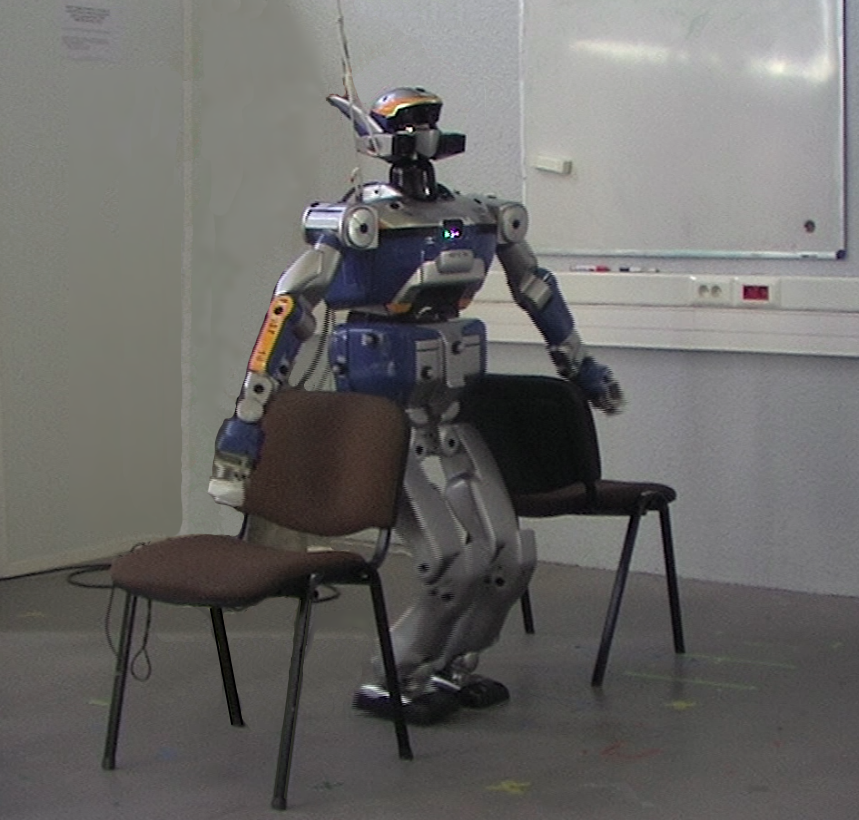
\includegraphics[width=0.6\linewidth]{pics/chairs/couv.png}
\caption{The robot HRP-2 passing between two chairs. In this kind of
  environment whole-body collision avoidance is needed during
  locomotion.} 
\label{fig:couv}
\end{figure}

There are two main ways of using motion planners to generate dynamically balanced robotic motions.
The more general one is to plan in a robot dynamic space, see for example \cite{shkolnik2011bounding}. 
By taking into account both robot
configuration and velocity, motions that satisfy dynamic balance constraints can be generated
at a planning phase. When planning motion for humanoid robots, this is a particularly costly
approach, as the size of the space to explore is augmented with the robot velocity and footprint
positions. The other way is to first plan  a geometric path that can be approximated by a
dynamic trajectory in a second step \cite{yoshida-humanoids05}. The approach we present in this paper 
falls into the second 
category. Some feasible dynamic motions are inherently impossible to compute with this kind
of approach. For example, jumping motions cannot be generated by a purely geometric planner.

\textbf{In this paper, we present a planning algorithm that considers
  exact models of a humanoid robot and its environment. It is used to
  solve navigation and manipulation problems. Our planner is a
  two-step algorithm: a first collision-free path is computed in the
  space of quasi-statically balanced configurations, then this first
  path is approximated by a sequence of dynamic walking
  trajectories. The proof of correctness of the algorithm is based on
  the concept of small-space controllability. This property allows,
  under some assumptions, to approximate any \textit{non necessarily
    admissible} path, by a sequence of admissible trajectories. In our
  context we prove that dynamic walking makes humanoid robots
  small-space controllable. Our planner is designed for perfectly
  modeled indoor environments, where the floor is horizontal and
  flat. Also, because we do not explicitly compute footprint positions
  at the planning stage, our planner is unable to plan motions in
  which the robot steps over obstacles. These limitations are
  discussed in the paper.}

\subsection{Outline}
Section~\ref{sec:related} reviews the related work and states our contribution. 
Section~\ref{sec:wb} presents a constrained motion planning algorithm, and its
use on a humanoid robot manipulation problem. Section~\ref{sec:wb-step} generalizes
the previous algorithm to problems that require locomotion. The generalization is
well-grounded, and
based on a controllability property of legged robots demonstrated in the paper. 
Section~\ref{sec:exp} presents some experimental results, and 
Section~\ref{sec:limits} discusses the limitations and potential future work of our
method.


\section{Related Work and Contribution}
\label{sec:related}


This work is based on several fields of humanoid robotics research:
prioritized inverse kinematics, randomized whole-body motion planning
and walk pattern generators based on the Zero-Moment Point (ZMP). This
section summarizes the literature related to each of these fields.

\subsection{Prioritized Inverse Kinematics}

The problem of inverse kinematics for a humanoid robot, or any articulated
structure, is to compute a joint position to achieve an end-effector pose. As the
robots we deal with are redundant, it is natural to take advantage of
this redundancy by specifying multiple tasks, potentially with
different priorities. This problem has been widely studied in robotics
planning and control literature, and many Jacobian-based solutions have been
proposed, among which 
\cite{nakamura1986iks}, \cite{siciliano1991gfm},
\cite{baerlocher1998tpf} and \cite{khatib2004wbd}.
Obstacle avoidance can be taken into account with similar methods. To
do so, one has to include the obstacles as  constraints to
satisfy, see for example \cite{kanehiro2008lca}.
These methods are prone to fall into local minima, thus global motion
planning is needed to overcome this limitation. 
{\bf Note that when local methods find solutions, these are usually smoother
and may look more natural. The choice of using global motion planners
is justified by the need for complete algorithms.}
\cite{TouGieGoe2007} propose a motion generation method where tasks follow
trajectories defined by cubic B-splines. The whole-body motion is optimized
with respect to the control point positions. This method can take into account
collisions with simple obstacles.

\subsection{Whole-Body Motion Planning}

When  planning a  whole-body motion  for a  humanoid robot, one difficult
challenge is to cope with  the curse of dimensionality. The complexity
of   motion  planning  is   exponential  in   the  dimension   of  the
configuration  space ($\mathcal{C}$)  to explore.  When  dealing with
high-dimensional configuration  spaces, it is  typically impossible to
explicitly represent  them, leading to the use  of randomized sampling
techniques  to solve  global planning  problems. In  the  past fifteen
years,  \textit{Probabilistic Roadmaps} \cite{kavraki1996prp} and  
\textit{Rapidly exploring Random  Trees} (RRT) 
\cite{kuffner00rrtconnect}  have been  developed and  used to  solve many
high-dimensional   planning  problems, see \cite{Lav06} and \cite{choset2005prm} for comprehensive
overviews.
When  using  sampling  techniques  on  a humanoid  robot,  another difficulty
is to  take into  account balance  constraints,  i.e. to
generate  random  configurations   on  zero  volume  submanifolds  of
$\mathcal{C}$. This problem has been investigated with success during
the last few years, \cite{Berenson15032011} presents an exhaustive survey
of Jacobian-based methods. Other recent contributions \cite{porta2012randomized}
present sophisticated constrained motion planning techniques based on higher-dimensional
continuation. Section \ref{sec:wb} presents a simple adaptation
of the RRT algorithm to constrained motion planning, that was first
introduced in \cite{dalibard09}.

\subsection{Walk Pattern Generation}

Another field of humanoid robotics research is the generation of
dynamically balanced walk patterns. Since the introduction of the ZMP
\cite{vukobratovic1969contribution}, several methods have been
proposed to generate walking motions efficiently.  One way to deal
with the complexity of a humanoid robot kinematic tree is to use the
so-called "cart-table" simplified model \cite{kajita2003biped}. Based
on this model, planning a trajectory for the ZMP is reduced to
planning a trajectory for the Center of Mass (CoM) of the robot.
Given a trajectory of the CoM and footprint positions, inverse
kinematics solvers can animate the whole set of DoFs of the robot to
generate a dynamically balanced walk trajectory.


\subsection{Collision-Free Walk Planning}

Collision-free  locomotion   trajectories  are  usually   obtained  by
simplifying the model of either the  robot or the environment. By reducing 
a  humanoid robot to a bounding volume that wraps the swaying motion,
one can  use a simple  planar motion planner  on this bounding  volume and
generate  a valid  locomotion  trajectory. This  strategy  is used  in
\cite{pettre20032} in a computer animation context. Variants of this method
include  dynamic path reshaping  \cite{yoshida-humanoids05}: if  collisions appear
when animating  the locomotion  trajectory, it is  locally reshaped
and re-animated.  This two-stage  strategy does not guarantee that the
locomotion trajectory can be followed or that the local reshaping will
converge.

\textbf{One possible simplification of the environment consists in
  considering obstacles at a footstep level only.
  \cite{kuffner2001footstep,chestnutt2005footstep,kuffner2005motion}
  use an A$^{*}$ algorithm to find collision-free footsteps.}  In
\cite{perrin2012fast}, the authors compute dynamic walking motions
avoiding collisions at the leg level by using an RRT algorithm.

Some planning methods for free-climbing robots \cite{bretl2006motion}
can be seen as a general way to consider quasi-static multi-step
planning. They are not however directly applicable to humanoid
dynamically balanced locomotion.  Other recent contributions to the
field of locomotion planning include algorithms considering the
dynamics at the planning phase \cite{shkolnik2011bounding}. This leads
to a growth of algorithmic complexity, particularly costly for
high-dimensional systems such as humanoid robots. To the authors'
knowledge such techniques have not been used on humanoid robotic
platforms so far.

\textbf{We show in this work that, under some assumptions, it is
  sufficient to plan a first path in the quasi-static configuration
  space of a humanoid robot, and then use the small-space
  controllability property to approximate this path by an admissible
  trajectory, i.e. a dynamically balanced walking motion. This result
  was first presented in \cite{dalibard2011small}.}

\subsection{Contribution}

The main contribution of this work is a whole-body motion planner for
humanoid robots that computes collision-free walking trajectories,
based on exact models of both robot and environment. It is used to
solve manipulation tasks that may require walking. The first stage of
our algorithm uses a sampling-based constrained motion planner and
computes a collision-free statically balanced path for a robot which
can be fixed or sliding on the ground.

Another contribution of this paper is the formal proof that dynamic
walking makes humanoid robots small-space controllable, with the
direct implication that this first path can always be approximated by
a dynamically balanced, collision-free walking trajectory. We have
implemented this well-grounded method, and the results have been
validated on the HRP-2 robot.

\section{Randomized Motion Planning on Constraint Manifolds}
\label{sec:wb}

\textbf{This section presents an algorithm for constrained motion
  planning on a submanifold $\manifold$ of the configuration space
  $\mathcal{C}$. In the particular case of a humanoid robot which is
  an under-actuated system, $\mathcal{C}=\mathcal{Q} \times SE(3)$,
  where $\mathcal{Q}$ represents the kinematic tree actuators and
  $SE(3)$ represents the position in space of the root of the tree. If
  the robot has $n$ actuated DoFs, then $dim(\mathcal{Q})=n$ and
  $dim(\mathcal{C})=n+6$. A configuration $q$ of $\mathcal{C}$ is said
  to be valid iff, besides being collision-free, it lies on the
  manifold $\manifold$; we call $\manifold$ the planning manifold.}

The problem solved here differs from classic approaches in two ways:
\begin{enumerate}
\item the set of valid configurations is defined implicitly, as the
  set of collision-free configurations satisfying a given set of
  inverse kinematics balance constraints;
\item the goal manifold $\goalmanifold$ is also defined implicitly,
  by additional inverse kinematics constraints.
\end{enumerate}
During global planning, we will consider several types of constraints
for various reasons:
\begin{itemize}
\item \textbf{Static balance: the CoM of the robot stays above the support
  polygon center, the two feet are horizontal on the ground.}
\item End-effector position and orientation: the goals of some problems presented
  in the experimental section of this paper are defined as a specific robot hand pose,
  or a gaze direction.
\item Configuration task: our adaptation of randomized motion planning algorithms 
  uses tasks defined as the distance towards a given configuration in $\mathcal{C}$. 
  This will be detailed in the following section.
\end{itemize}


Our algorithm generalizes randomized tree expansion strategies, introduced in both \cite{HsuLat99c} and
\cite{kuffner00rrtconnect} to constrained motion planning problems. Next subsection will recall the structure of the RRT algorithm,
a popular randomized motion planning algorithm. 
{\bf Our method could be applied to any randomized sampling planning method, such
as RRT\textsuperscript{*} \cite{Karaman01062011}, which is slower than RRT but generates optimal
paths.}


\subsection{Rapidly exploring Random Trees (RRT)}

The classic RRT algorithm, as presented in  \cite{kuffner00rrtconnect}, grows 
a random tree inside the robot 
collision-free configuration space 
$\mathcal{C}_{free}$. Each iteration of the algorithm attempts to extend the tree
by adding new vertices in the direction of a randomly selected configuration
$q_{rand}$. Algorithm~\ref{algRRT} shows the pseudo-code of the RRT algorithm.
It takes as input an initial configuration $q_0$ and grows a tree  $\mathcal{T}$ rooted 
in $q_0$. 

\begin{algorithm}
\caption{RRT($q_0$)}
\label{algRRT}
\begin{algorithmic}
\STATE $\mathcal{T}.$Init$(q_0)$
\FOR{$i$ = 1 to $K$}
\STATE $q_{rand} \leftarrow $ Rand$(\mathcal{C})$
\STATE $q_{near} \leftarrow $ Nearest$(q_{rand},\mathcal{T})$
\STATE Extend$(\mathcal{T},q_{near},q_{rand})$
\ENDFOR

\end{algorithmic}
\end{algorithm}

One way to make the RRT algorithm more efficient is to grow trees from both the initial
and  goal configurations. This was first proposed in 
\cite{kuffner00rrtconnect}. Our formulation of manipulation planning does
not include an explicit goal configuration, so it is not possible to directly grow
a tree from the goal. To make use of the idea of growing multiple trees, we first
randomly sample the goal manifold and generate several goal configurations. Then, 
we grow random
trees from the initial configuration and the random goal configurations. The idea of
generating several goals for manipulation planning was proposed in \cite{diankov2008bpc}.

Section~\ref{sec:SolveConstraints} describes a constraint solver,
Section~\ref{sec:goal-sampling} the goal manifold sampling, and
Section~\ref{sec:extension} the adaptation or RRT random extensions to
constrained motion planning.

\subsection{Constraint Solver}
\label{sec:SolveConstraints}

\textbf{We show here how a multiple constraint solver works: its
  purpose is to find the root $q$ of a non-linear $C^1$ function
  $f(q)$ with a tolerance of $\epsilon$. If we want to find a
  configuration on a manifold $\manifold$, $f(q)$ can be defined as a
  vector valued function that contains the concatenation of all
  constraints defining $\manifold$. Note that as the intersection of
  two or more manifolds is also a manifold, this constraint solver
  allows us also to generate configurations that lie at the
  intersection of several manifolds.}

\textbf{Algorithm~\ref{algo:newton} implements a Newton-Raphson method
  \cite{bonnans2006numerical}: starting from an initial value of $q$,
  $q$ is updated iteratively by $- \alpha \left(\frac{\partial
    f}{\partial q}(q)\right)^{+} f(q)$, where $\alpha$ denotes a gain
  and $\left(\frac{\partial f}{\partial q}(q)\right)^{+}$ denotes the
  Moore-Penrose pseudo-inverse of the Jacobian of $f(q)$. The use of
  an adaptive gain $\alpha$, which increases iteratively from an
  initial value $\alpha$ to a maximum value $\alpha_{max}$, allows the
  overshoot avoidance and convergence acceleration. The update rule
  relies on a real factor $w \in [0,1]$; the greater $w$ is, the
  faster $\alpha$ will reach $\alpha_{max}$. Obviously, the solver
  convergence depends on the initial value of $q$, and a bad
  initialization can lead to either slow convergence or failure. A
  cutoff number of iterations $it_{max}$ is hence introduced to bypass
  these cases.}

\textbf{We observed that values of $\epsilon=10^{-6}$,
  $\alpha=0.1$, $\alpha_{max}=0.95$ and $w=0.8$ lead to good behavior,
  i.e. fast convergence and low failure rate. These values are kept
  constant for all scenarios in this work.}

\begin{algorithm}
\caption{\texttt{SolveConstraints}($q$, f, $\epsilon$): find $q$
  such that $f(q) = 0$}
\label{algo:newton}
\begin{algorithmic}
\STATE $i=0$
\WHILE{$\|f(q)\| > \epsilon$ and $i\leq it_{max}$}
\STATE {\color{red} // $\left(.\right)^{+}$ denotes the Moore-Penrose pseudo-inverse}
\STATE $q \leftarrow$ $q - \alpha \left(\frac{\partial f}{\partial q}(q)\right)^{+} f(q)$
\STATE $i$ $\leftarrow$ $i+1$
\STATE {\color{red}// Make $\alpha$ tend toward $\alpha_{max}$}
\STATE $\alpha \rightarrow \alpha_{max} - w(\alpha_{max} - \alpha)$
\ENDWHILE
\IF {$\|f(q)\| \leq \epsilon$}
\STATE return $q$
\ELSE
\STATE return failure
\ENDIF
\end{algorithmic}
\end{algorithm}

\subsection{Goal Manifold Sampling}
\label{sec:goal-sampling}

The way we generate a goal configuration is the following:
\begin{enumerate}
\item \textbf{Shoot a random configuration $q_{rand}$ in $\mathcal{C}$ with
  uniform distribution.}
\item \textbf{Call \texttt{SolveConstraints} (Algorithm~\ref{algo:newton}) on
  $q_{rand}$, with $f(q)$ defined by the intersection of the planning
  and goal manifolds $\manifold \cap \goalmanifold$.}
\item If success, check for collisions.
\end{enumerate}

\textbf{Fig.~\ref{fig:goal} shows resulting random configurations
  which satisfy both balance ($\manifold$) and reaching
  ($\goalmanifold$) constraints for the HRP-2 robot.}

\begin{figure}[h]
\centerline {
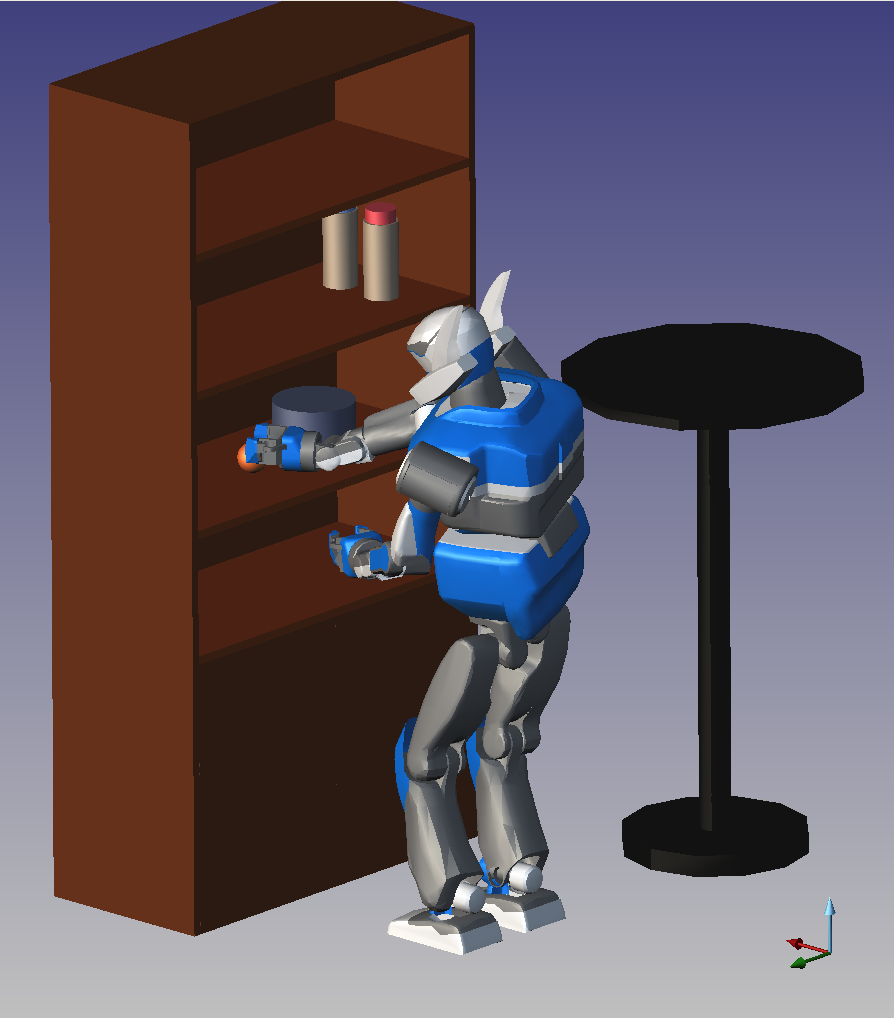
\includegraphics[width=.24\linewidth]{pics/goal-config/goal0.png}
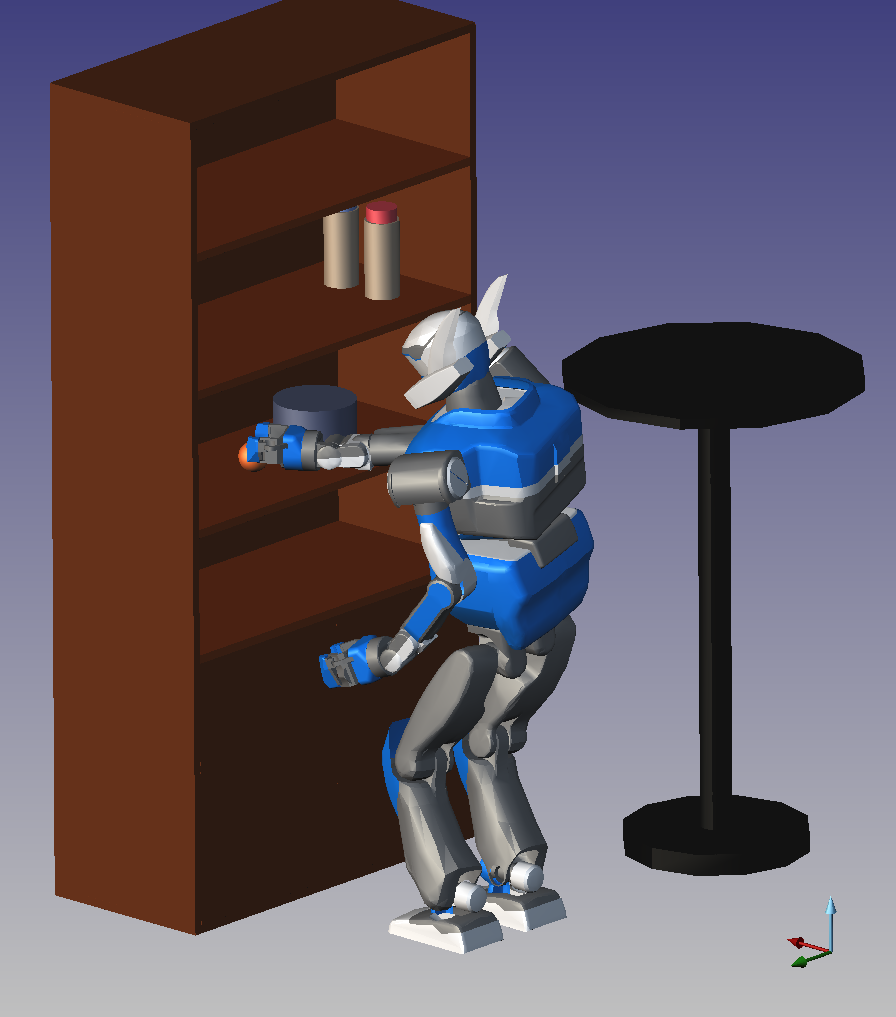
\includegraphics[width=.24\linewidth]{pics/goal-config/goal1.png}
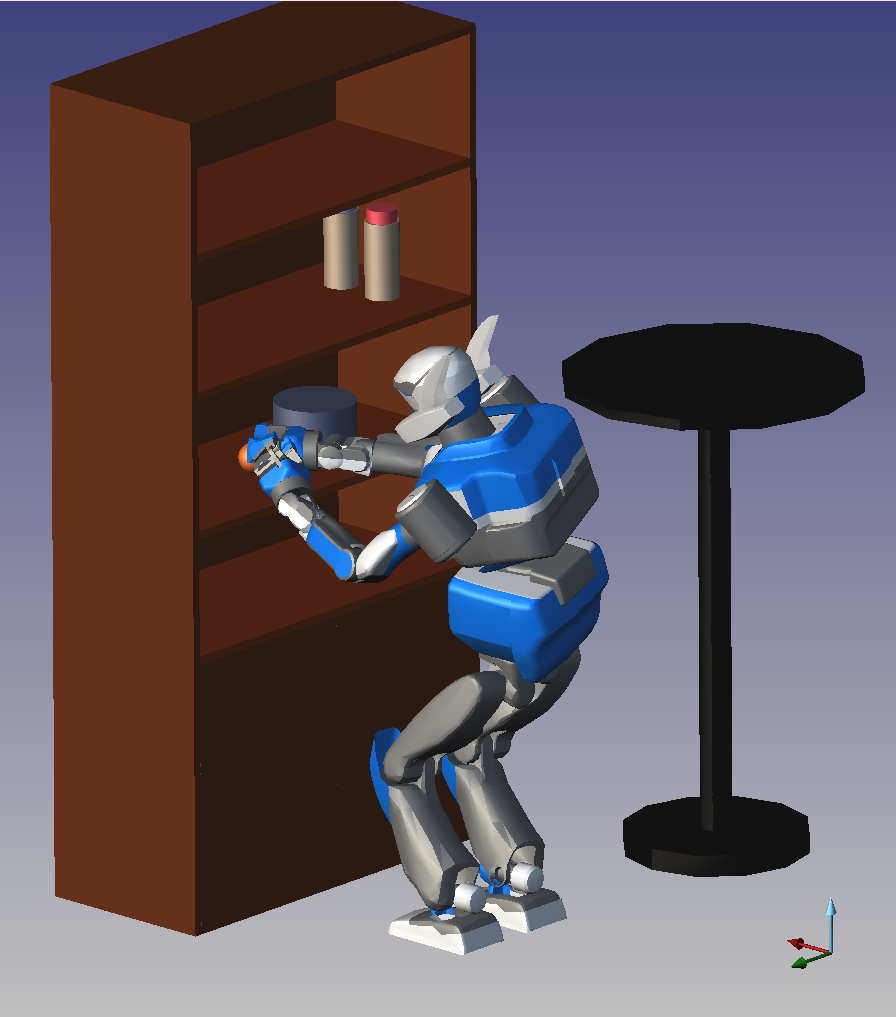
\includegraphics[width=.24\linewidth]{pics/goal-config/goal2.png}
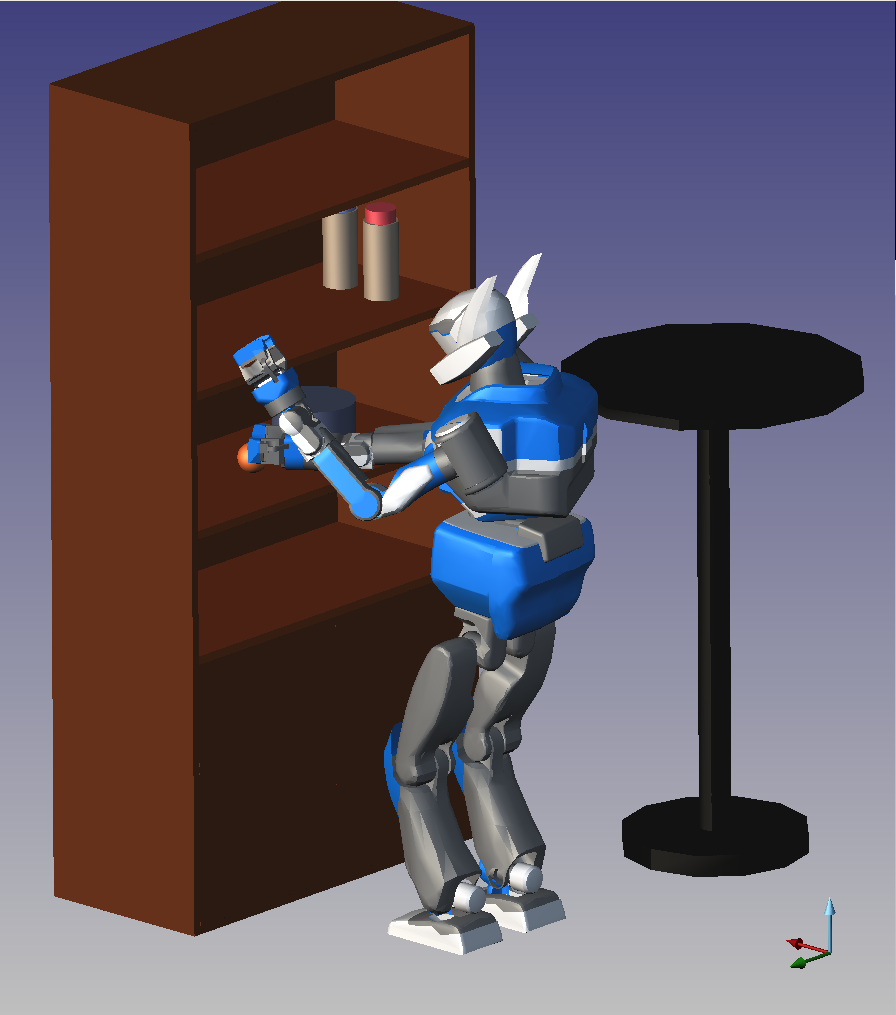
\includegraphics[width=.24\linewidth]{pics/goal-config/goal3.png}
}

\caption{Random goal configurations solving a reaching task. All the
  configurations are balanced and collision-free, and the right hand of the character
  reaches the orange ball.}
\label{fig:goal}
\end{figure}



\subsection{Random Extensions on a Constrained Manifold}
\label{sec:extension}



Fig.~\ref{fig:rrt-extend} shows an extension of the classic 
RRT algorithm, from a configuration already in the tree $q_{near}$ towards a random
configuration $q_{rand}$.

\begin{figure}[h]
  \centering

  \begin{tikzpicture}[x=0.45cm,y=0.45cm]

    \node [draw,circle,inner sep=2pt] (0) at (0,0) {};
    \node [draw,circle,inner sep=2pt] (1) at (1,1) {};
    \node [draw,circle,inner sep=2pt] (2) at (2.4,1) {};
    \node [draw,circle,inner sep=2pt,fill=gray] (qn) at (3.4,2) {};
    \node [above left] at (qn) {$q_{near}$};
    \node (t) at (1.5,-0.5) {$\mathcal{T}$};
    \draw (0) -- (1) -- (2) -- (qn) ; 

    \node [draw,circle,inner sep=2pt] (qn2) at (7.6,2) {};
    \node [above left] at (qn2) {$q_{new}$};

    \draw (qn) -- (qn2) ;

    \path[draw=black,line join=miter,line cap=butt,line width=0.800pt, fill=gray]
    (8,2) .. controls (8,4) and (10,6) ..
    (12,5) .. controls (14,4) and (14,4) ..
    (15,2) .. controls (15,0) and (14,0) ..
    (13,0) .. controls (11,1) and (8,1) ..
    (8,2) -- cycle;


    \node [draw,circle,inner sep=2pt,fill=white] (qrand) at (13,2) {};
    \node [below] at (qrand) {$q_{rand}$};

    \node at (10.5,4) {Obstacle};
    

    \draw [dashed,thin] (qn2) -- (qrand) ;



  \end{tikzpicture}

  \caption{One step of extension of the RRT algorithm. The algorithm tries to add the longest possible edge
  from $q_{near}$ towards $q_{rand}$, while avoiding collisions.} 
  \label{fig:rrt-extend}
\end{figure}

The equivalent random extension on a constrained manifold $\manifold$,
defined by the constraint function $f$, starts from a valid
configuration $q_{near} \in \manifold$, and extends the tree towards a
random configuration $q_{rand}$, while keeping the constraints
satisfied. Extension attempts orthogonal to $\manifold$ are useless,
as newly added edges have to be included in $\manifold$. To extend in
directions that follow the directions of $\manifold$, we rely on
Jacobian-based inverse kinematics. Algorithm~\ref{alg:constrained}
presents the adaptation of the classic extend function, and
Fig.~\ref{fig:gikrrt} illustrates this extension. The idea is to first
project $q_{rand}$ on the tangent space to $\manifold$ at
$q_{near}$. Let us call the projected configuration $q_{rand}'$. Let
$q_{rand}''$ be the result of a call to
$\texttt{SolveConstraints}(q_{rand}',f,\epsilon)$.  It is the
projection of $q_{rand}'$ on $\manifold$. Instead of extending the
tree from $q_{near}$ towards $q_{rand}$, the algorithm tries to extend
from $q_{near}$ towards $q_{rand}''$ while remaining on
$\manifold$ \footnote{This presentation attempts to give a precise
  idea of the algorithm, without focusing on technical
  details. Readers interested in the actual implementation can refer
  to \url{https://github.com/laas/hpp-constrained} and
  \url{https://github.com/laas/hpp-constrained-planner}, where the
  corresponding open-source code is available.}. While extending the
tree, the configurations along the new edge are automatically
projected onto $\manifold$. These projections are not very costly if
the edge is close to the constrained manifold. 

{\bf \cite{berenson2011task} presents a formal proof that projection-based 
constrained random motion planning on a fixed dimension manifold is 
probabilisticaly complete. This proof applies to our algorithm. }


\begin{figure}[h]
\centering
\begin{minipage}[c]{0.6\linewidth}
\begin{tikzpicture}[y=0.55pt, x=0.55pt,yscale=-1, inner sep=0pt, outer sep=0pt]
\definecolor{dg}{rgb}{0,0.3,0}
\path[draw=black,line join=miter,line cap=butt,line width=0.800pt, fill=gray]
  (231.3249,143.2249) .. controls (178.0814,153.1889) and (178.5527,172.4247) ..
  (180.8173,200.8036) .. controls (183.2959,231.8645) and (195.6610,188.6038) ..
  (256.5787,230.0980) .. controls (295.8993,256.8813) and (346.4296,308.3911) ..
  (295.9747,178.5802) .. controls (275.5517,126.0356) and (304.8066,129.4735) ..
  (231.3249,143.2249) -- cycle;
\node at (230,180) {Obstacle};
\path[dashed,draw=dg,line join=miter,line cap=butt,line width=1.5pt]
  (88.8934,277.5752) .. controls (196.3490,276.5363) and (532.8532,213.7494) ..
(434.3656,81.6056) node [above = 0.1cm, color=dg, text width=1.8cm] {\small{Constrained manifold $\manifold$}};
\node [draw,circle,inner sep=2pt,fill = gray] (qn) at (97,277) {};
\node [above = 0.15cm] at (qn) {$q_{near}$};
\node [draw,circle,inner sep=2pt] (qr1) at (367,99) {};
\node [left = 0.2cm] at (qr1) {$q_{rand}$};
\draw [dashed,thin] (qn) -- (450,277);
\node [right = 0.2cm] at (450,277) {\small{$T_q\manifold$}};
\node [draw,circle,inner sep=2pt] (qr2) at (367,277) {};
\node [below right = 0.1cm] at (qr2) {$q_{rand}'$};
\node [draw,circle,inner sep=2pt,fill = gray] (qr3) at (345,225) {};
\node [above = 0.22cm] at (qr3) {$q_{rand}''$} ;
\draw [dashed,thin] (qr1) -- (qr2) -- (qr3);
\node [draw,circle,inner sep=2pt,fill = gray] (qnew) at (270,250) {};
\node [above = 0.1cm, left = 0.2cm] at (qnew) {$q_{new}$};
%\draw [thick] (qn) -- (qnew);

\end{tikzpicture}
\end{minipage}
\begin{minipage}[c]{0.3\linewidth}
%% \begin{tikzpicture}[x=0.61cm,y=0.61cm]
%%    \definecolor{dg}{rgb}{0,0.3,0}
%%       %Stack of tasks:
%%       \draw [color=black, thick,fill = white] (0,1) rectangle (2,2);
%%       \draw [color=black, thick,fill = white] (0,2) rectangle (2,3);
%%       \draw [color=black, thick,fill = white] (0,3) rectangle (2,5);
%%       \draw [color=black, thick,fill = white] (0,5) rectangle (2,6);
%%       \draw [color=black, thick,fill = white] (0,6) rectangle (5,7);
%%       \draw [color=black, thick,fill = white] (1,1) rectangle (5,6);
%%       \draw [thick] (1,1) -- (5,1) -- (5,6);
%%       \draw (1,2) -- (5,2) ;
%%       \node [text width = 5cm,text centered] at (2.5,6.5) {\large Stack
%%         of tasks};
%%       \begin{scriptsize}
%%         \node at (0.5,5.5) {1};
%%         \node at (0.5,4) {$\vdots$}; 
%%         \node at (0.5,2.5) {$n$};
%%         \node at (0.5,1.5) {$n$+1};

%%         \node [text width = 2cm,color=dg] at (3.2,4) {\small Constraints defining
%%           $\manifold$};
%%         \node [text width = 3cm,text centered] at (3,1.5)
%%               { Configuration task towards $q_{rand}$};    
%%       \end{scriptsize}


%% \end{tikzpicture}
\end{minipage}

\caption{\textbf{One step of constrained extension illustrating
    Algorithm \ref{alg:constrained}: $q_{rand}$ is first projected on
    $T_q\manifold$ the tangent space of $\manifold$. $q_{rand}'$ is
    then projected onto $\manifold$. A classic RRT extension tries to
    go as far as possible from $q_{near}$ towards $q_{rand}''$ while
    remaining on $\manifold$. $q_{new}$ is then returned.}}
\label{fig:gikrrt}
\end{figure}

\begin{algorithm}[h]
  \caption{\texttt{ConstrainedExtend}($\mathcal{T},q_{near},q_{rand},f,\epsilon$)}
  \label{alg:constrained}
  \begin{algorithmic}
    \STATE $d \leftarrow$ \texttt{Distance}($q_{near}, q_{rand}$)
    \STATE $q \leftarrow$ $q_{near}$
    \WHILE{$d > \epsilon$}
    \STATE $q_{rand}' \leftarrow$ \texttt{OrthogonalProject}($q_{rand}, T_q\manifold$)
    \STATE $q_{rand}'' \leftarrow$ \texttt{SolveConstraints}($q_{rand}',f,\epsilon$)
    \STATE $d \leftarrow$ \texttt{Distance}($q,q_{rand}''$)
    \STATE $q \leftarrow q_{rand}''$
    \ENDWHILE
    \STATE $q_{new} \leftarrow$ RRT::Extend($\mathcal{T},q_{near},q_{rand}''$)
  \end{algorithmic}
\end{algorithm}
    
\subsection{Example}

\textbf{We present in Fig.~\ref{fig:wb-shelves} an illustration of the
  use of randomized motion planning on complex manipulation
  problems. The humanoid robot HRP-2 faces shelves. It has to: (i)
  grasp a ball lying on a shelf, (ii) put it on a higher shelf, (iii)
  come back to a natural rest configuration. We can hence define three
  separate constrained motion planning problems where the planning
  manifold $\manifold$ is the static balance manifold defined in
  \ref{sec:wb}; the goal manifold of problem (i) is defined by a hand
  pose constraint (the hand must be horizontal and its position has to
  coincide with the ball initial position), and a gaze constraint (the
  robot has to look at the ball in its initial position). Similarly,
  the goal manifold of problem (ii) is defined by hand and gaze
  constraints that correspond to the position of the ball on the
  higher shelf. Finally, we define the rest configuration as the
  single goal configuration for problem (iii).}

\textbf{Note that for phases (i) and (iii) the ball is also considered
  as an obstacle. This is necessary to prevent the robot grasping hand
  from colliding with the ball during the approach (respectively
  retraction) phase.}

\textbf{For the two reaching motions in (i) and (ii), we first
  generate 8 random goal configurations
  (Section~\ref{sec:goal-sampling}), then we solve the three
  constrained motion planning problems separately. As randomized
  motion planning algorithms produce, a classic shortcut method is
  used to optimize and shorten the paths. Extension 1 presents a
  video of the concatenated motion.}

\textbf{We have run this set of motion planning problems 20 times;
  results are compiled in Table~\ref{table:reaching}. We have also
  measured the performance of \texttt{SolveConstraints} (Algorithm
  \ref{algo:newton}) when used to project configurations on
  $\manifold$; the average number of iterations is 6.5 per call, and
  the success rate, i.e. the ratio of the number of successfully
  projected configurations over the total number of calls, is above 95
  percent. This success rate, high as it is, could be further improved
  by sampling a better initial configuration of $\mathcal{C}$, for
  example by introducing a heuristic bias towards statically balanced
  configurations. Nevertheless we choose to sample $\mathcal{C}$
  uniformly-randomly for the sake of genericity.}

\begin{figure}[h]
\centering
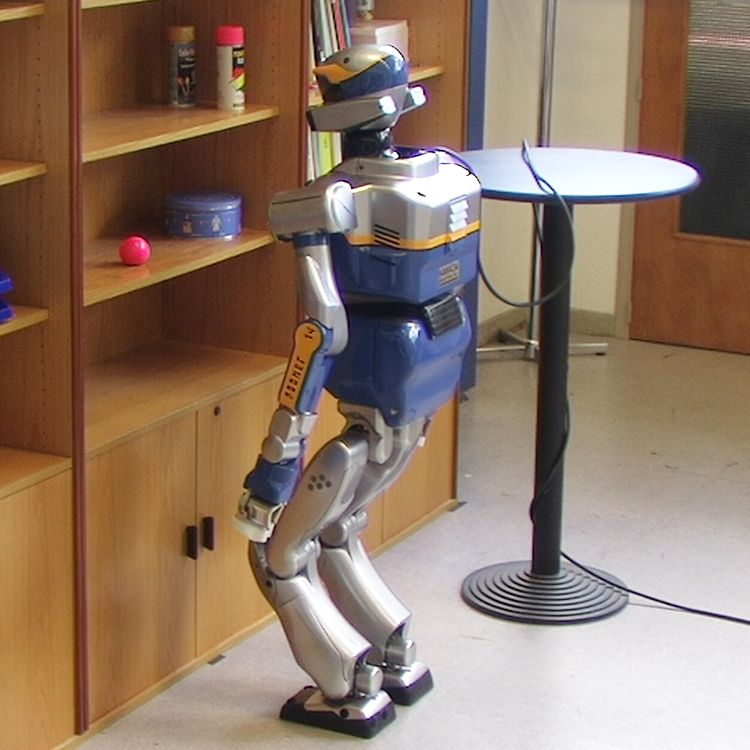
\includegraphics[width=0.24\linewidth]{pics/wb-shelves/1.jpg}
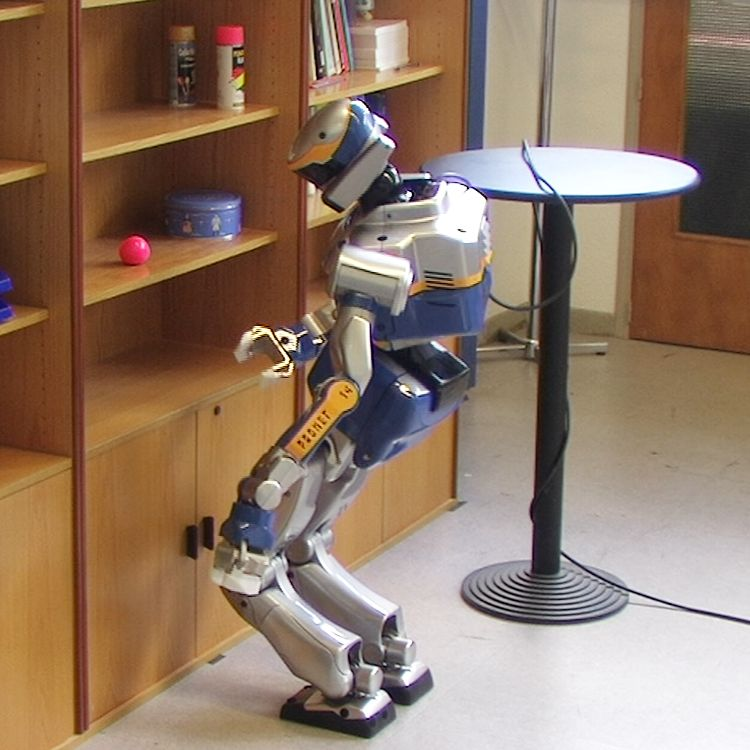
\includegraphics[width=0.24\linewidth]{pics/wb-shelves/2.jpg}
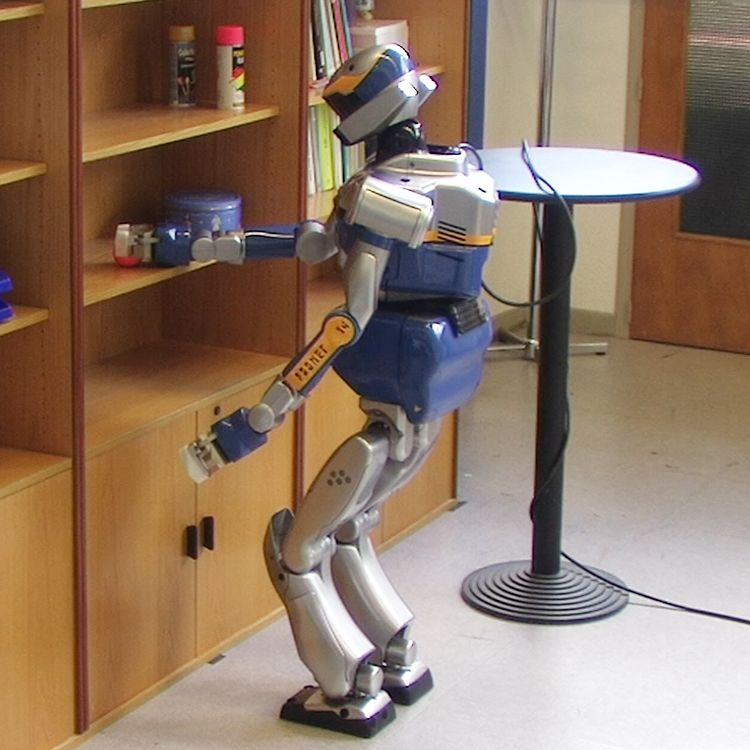
\includegraphics[width=0.24\linewidth]{pics/wb-shelves/3.jpg}
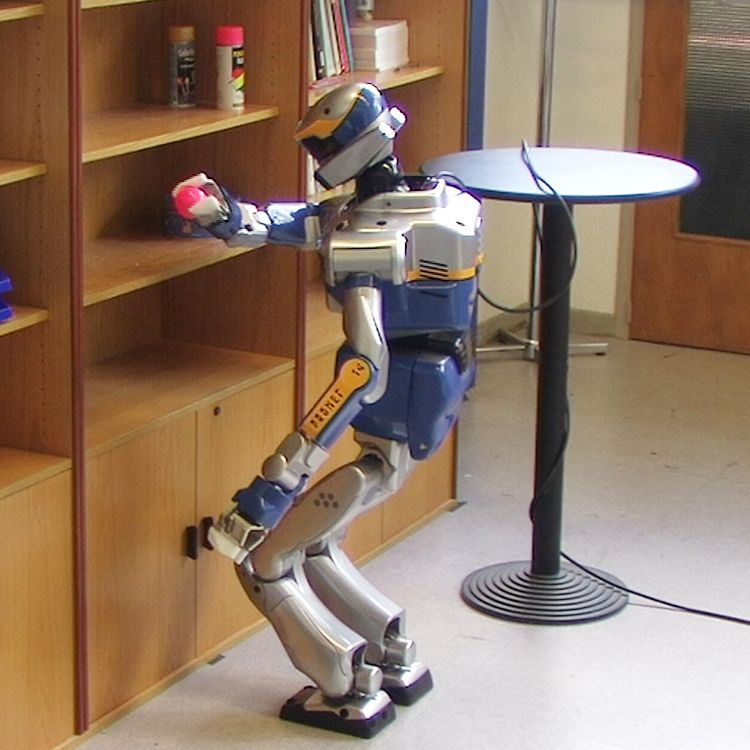
\includegraphics[width=0.24\linewidth]{pics/wb-shelves/4.jpg}
\\
\vskip 0.08cm
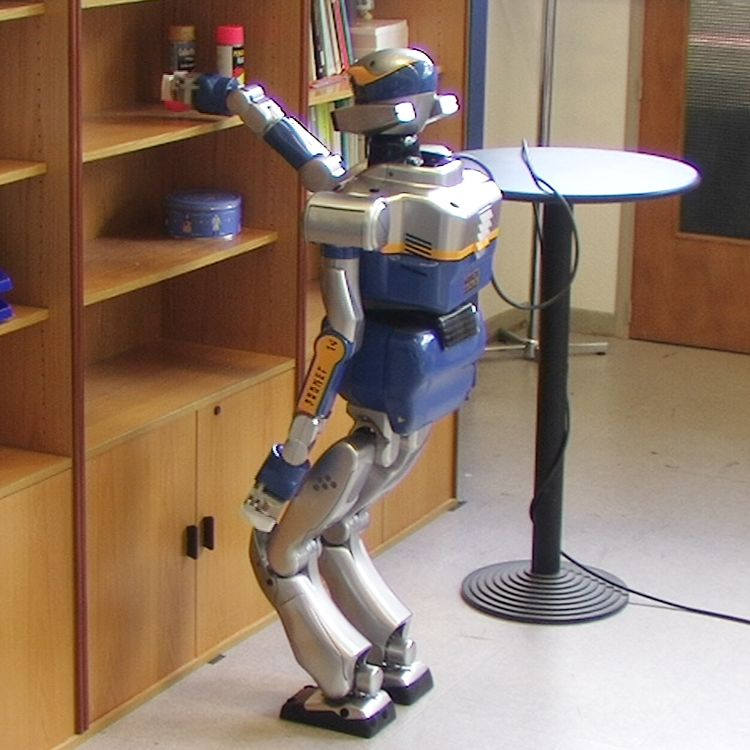
\includegraphics[width=0.24\linewidth]{pics/wb-shelves/5.jpg}
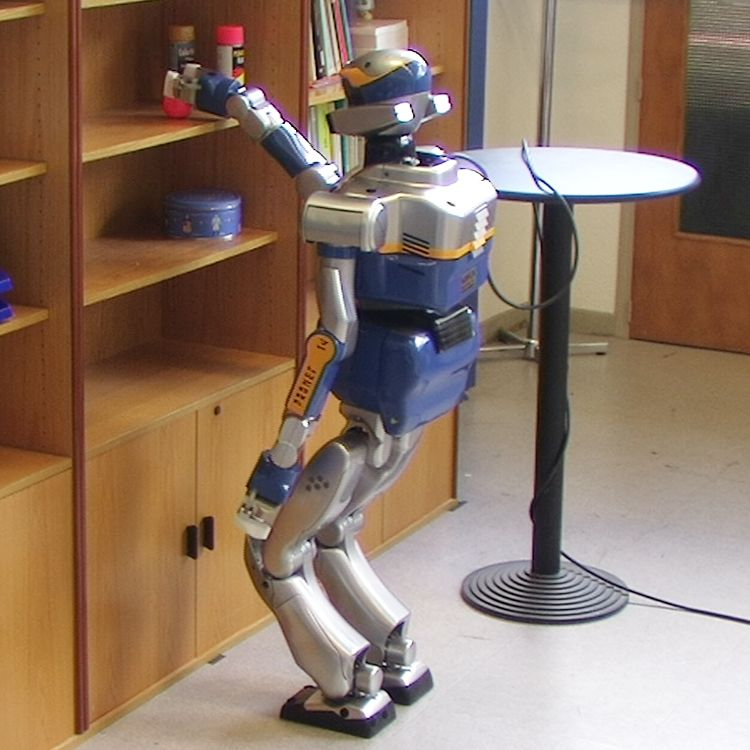
\includegraphics[width=0.24\linewidth]{pics/wb-shelves/6.jpg}
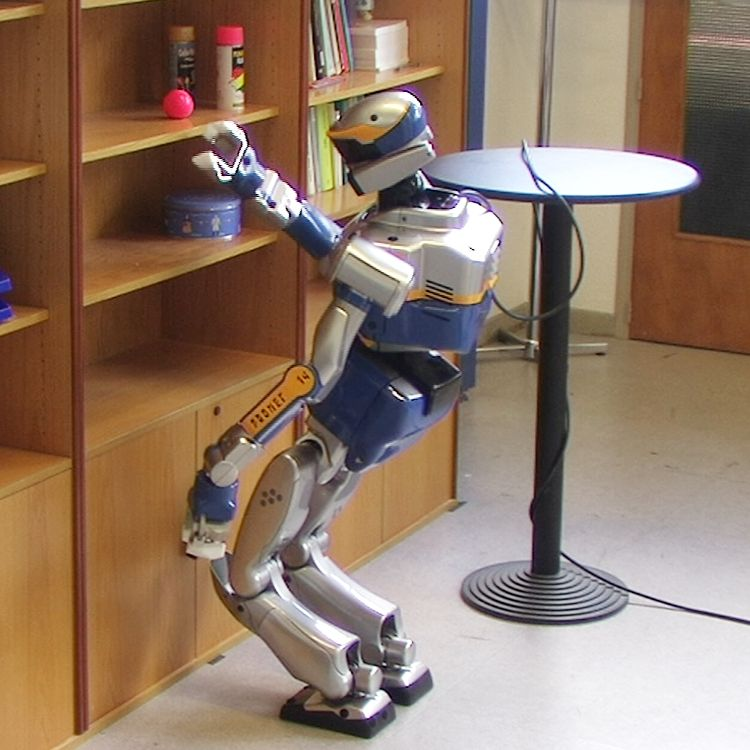
\includegraphics[width=0.24\linewidth]{pics/wb-shelves/7.jpg}
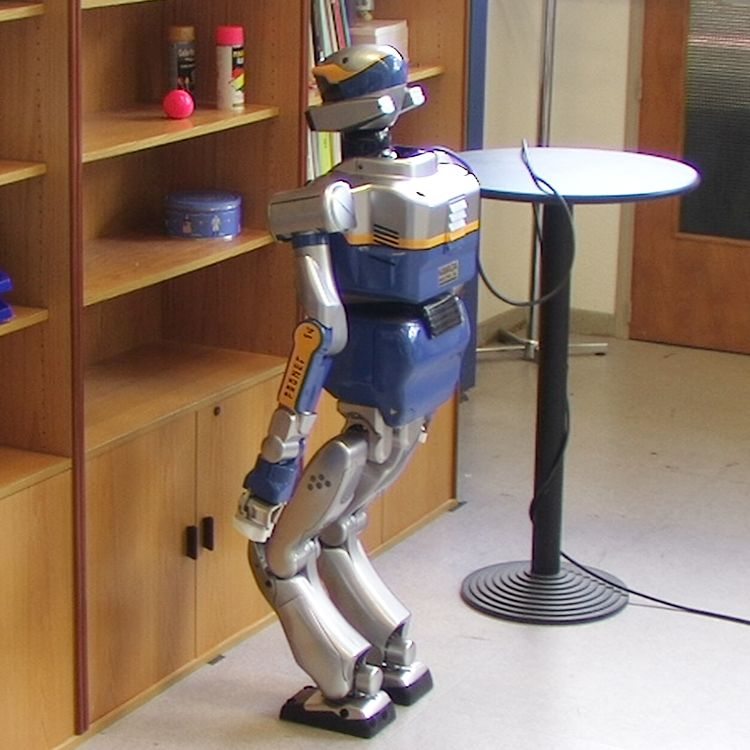
\includegraphics[width=0.24\linewidth]{pics/wb-shelves/8.jpg}

\caption{HRP-2 grabs a ball on a shelf, puts it on another shelf, and comes back to 
  a rest position. Static balance constraints are enforced along the path, and 
  the intermediary goals consisting in grasping and displacing the ball are defined
  implicitly as inverse kinematics constraints.}
\label{fig:wb-shelves}
\end{figure}

\begin{table}
\begin{tabular}{l|r|r|r|r|}
\cline{2-5}
& min & max & average & average \\ 
&&&& per problem \\
\hline
\multicolumn{1}{|l|}{number of nodes} & 43.00 & 481.00 & 102.70 \\
\cline{1-4}
\multicolumn{1}{|l|}{goal generation time (s)} & 1.00 & 1.56 & 1.22\\
\hline
\multicolumn{1}{|l|}{planning time (s)} & 67.36 & 376.84 & 134.28 & 44.76\\
\hline
\end{tabular}
\caption {\textbf{Experimental results on 20 runs: Each run consists
    of 3 motion planning problems and 2 goal generations for the three
    phases. Time is expressed in seconds.}}
\label{table:reaching}
\end{table}

\section{From Statically Balanced Paths to Dynamic Walk Trajectories}
\label{sec:wb-step}

The previous section has presented a simple algorithm that solves
manipulation planning problems on a given constraint manifold
$\manifold$ of $\mathcal{C}$.

If we use this algorithm with static balance constraints without
fixing globally the robot foot positions, it generates statically
balanced paths for a robot \textit{sliding} on the
ground. \textbf{Fig~\ref{fig:sliding} shows an example of a whole-body
  collision-free path for a robot passing between two chairs. Since in
  reality a legged robot cannot slide on a regular floor, such paths
  are physically unfeasible. They are, however, easier to generate
  than feasible dynamic walking trajectories because only geometric
  constraints are considered at planning time.}

\begin{figure}[h]
  \centering

  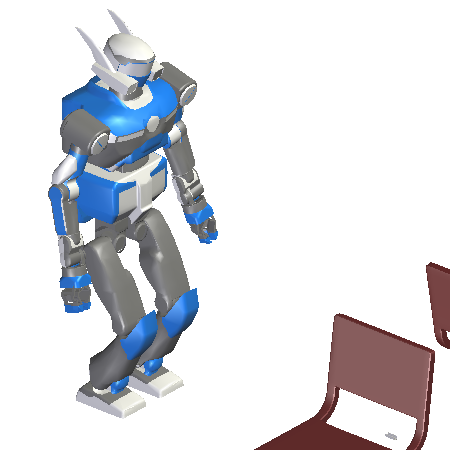
\includegraphics[width=0.24\linewidth]{pics/chairs/sliding-perspective-1.png}
  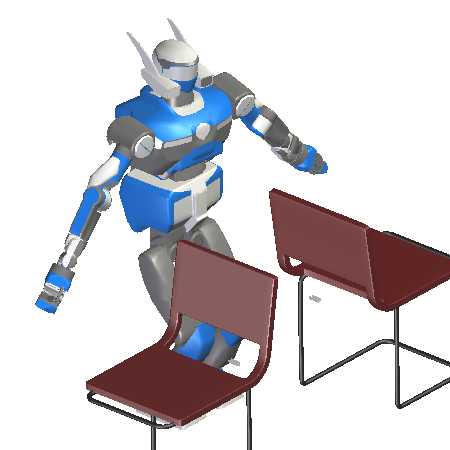
\includegraphics[width=0.24\linewidth]{pics/chairs/sliding-perspective-2.png}
  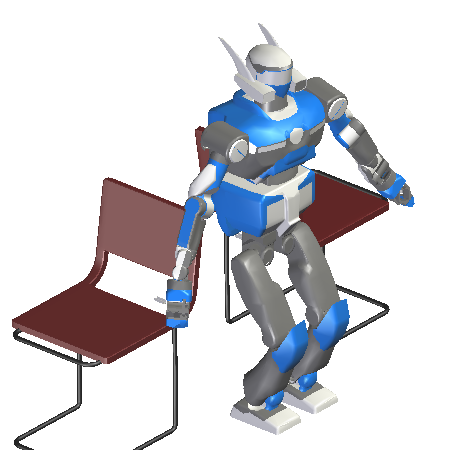
\includegraphics[width=0.24\linewidth]{pics/chairs/sliding-perspective-3.png}
  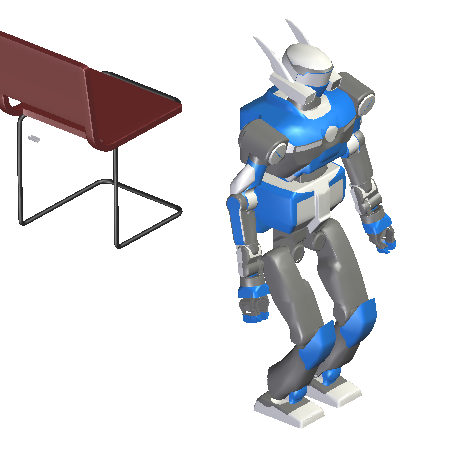
\includegraphics[width=0.24\linewidth]{pics/chairs/sliding-perspective-4.png}


  \caption{Collision-free  statically balanced path  for a  humanoid  robot  sliding on  the
    ground.}
  \label{fig:sliding}
\end{figure}



This section presents a \textit{constructive} proof that any such statically balanced, 
collision-free path for a legged robot sliding
on the ground can be approximated by a  dynamically balanced, collision-free walk trajectory.
The proof is based on ideas from control theory, in particular small-space 
controllability. It also uses the fact that balance criteria for dynamic walking are different
from the ones for static balance. 

Section~\ref{sec:ssc} recalls the definition of small-space controllability and its
use in motion planning. Section~\ref{sec:humanoid-ssc} proves that a
dynamically walking legged robot is small-space controllable, while a quasi-statically
walking legged robot is not. Section~\ref{sec:ssc-application} shows how this property is used to
approximate collision-free statically balanced paths by dynamic walking trajectories.


\subsection{Small-Space Controllability}
\label{sec:ssc} 

A  robotic system  is  controllable  if  for any two  configurations
$q_1$ and $q_2$,  there exists  a
trajectory  going  from  $q_1$ to  $q_2$.  It  is  
\textit{small-space  controllable} if for all configurations  $q$, 
for all $\epsilon >0$, there
exists $\eta >0$ such that all the configurations contained in the ball of center
$q$ and radius $\eta$ are reachable by trajectories included in the
ball of center $q$ and radius $\epsilon$. Fig.~\ref{fig:ssc1} shows an illustration
of this property.

\begin{figure}[h]
  \centering
  
\definecolor{cc6c6c6}{RGB}{198,198,198}
\definecolor{cffffff}{RGB}{255,255,255}

\begin{tikzpicture}[y=0.4pt, x=0.4pt,yscale=-1, inner sep=0pt, outer sep=0pt]
% path5273
\path[shift={(-0.42857142,4.7142857)},draw=black,miter limit=4.00,line
  width=0.800pt]
  (365.7143,269.5050)arc(0:180:97)arc(-180:0:97) --
  cycle;

% path5275
\path[shift={(-6.0609153,-3.535534)},draw=black,fill=cc6c6c6,miter
  limit=4.00,line width=0.800pt]
  (323.7539,278.0803)arc(-0:180:51)arc(-180:0:51) --
  cycle;

% path5315
\path[draw=black,line join=miter,line cap=butt,miter limit=4.00,line
  width=1.200pt] (265.6701,275.0498) .. controls (265.6701,275.0498) and
  (165.7228,265.2948) .. (178.2919,306.8696) .. controls (185.4208,330.4496) and
  (285.8732,311.9204) .. (285.8732,311.9204) -- (285.8732,311.9204);

% path4761
\path[draw=black,fill=cffffff,miter limit=4.00,line width=0.400pt]
  (278.8021,274.5447)arc(0:180:12)arc(-180:0:12) --
  cycle;

% path4761-4
\path[shift={(17.677674,33.840124)},draw=black,fill=black,miter limit=4.00,line
  width=0.400pt]
  (278.8021,274.5447)arc(-0:180:12)arc(-180:0:12) --
  cycle;

% text5307
\path[fill=black] (288,334.92981) node[right] (text5307) {$q'$};

% text5311
\path[fill=black] (280,286.9537) node[above right] (text5311) {$q$};

% path5319
\path[draw=black,fill=black,line join=miter,line cap=butt,line width=0.800pt]
  (201.0204,312.4254) -- (220.7183,318.9914) -- (200.5153,323.0320) --
  (201.0204,312.4254) -- cycle;

% path2829
\path[draw=black,line join=miter,line cap=butt,line width=0.800pt,<->]
  (273.5714,264.5050) -- (320.0,191.6479);

% path2831
\path[draw=black,line join=miter,line cap=butt,line width=0.800pt,<->]
  (254.2857,270.2193) -- (226.4286,245.2193);

% text2833
\path[fill=black] (302.14285,231.6479) node[above right] (text2833) {$\epsilon$};

% text2837
\path[fill=black] (242.14285,258.07648) node[above right] (text2837) {$\eta$};


\end{tikzpicture}


  \caption{The small-space controllability local property:  any configuration $q'$ 
    at a distance less than
    $\eta$ is reachable from $q$ by an admissible trajectory included in
    a ball of size $\epsilon$.}
  \label{fig:ssc1}
\end{figure}

The main  consequence of  this property  
in  motion planning  is the following theorem, that shows how planning for
dynamic systems is reduced to geometric planning
thanks to the small-space controllability property:

\begin{theorem}
  \label{thm:ssc}
  Any collision-free path of a small-space controllable system can be approximated
  by a sequence of both collision-free and admissible trajectories. Thus, small-space 
  controllability reduces trajectory planning problems to geometric path planning problems.
\end{theorem}

Fig. \ref{fig:ssc2} shows an example of collision-free 
path approximation by admissible collision-free sub-trajectories. The convergence 
of this algorithm is guaranteed by the small-space
controllability property.

\begin{figure}[h]
  \centering

  
\definecolor{cd9d9d9}{RGB}{217,217,217}
\definecolor{c888888}{RGB}{136,136,136}
\definecolor{cc8c8c8}{RGB}{200,200,200}

\begin{tikzpicture}[y=0.65pt, x=0.65pt,yscale=-1, inner sep=0pt, outer sep=0pt]
  \begin{scope}% layer1
    % path4348-7-9
    \path[cm={{0.88069687,0.0,0.0,0.88069687,(30.925926,8.8427197)}},draw=black,fill=cd9d9d9,miter
      limit=4.00,fill opacity=0.450,line width=0.273pt]
    (347.2399,152.3163)arc(0:180:14)arc(-180:0:14) --
    cycle;

    % path4348-7-9-7
    \path[cm={{1.1259005,0.0,0.0,1.1259005,(-41.191,-23.012876)}},draw=black,fill=cd9d9d9,miter
      limit=4.00,fill opacity=0.450,line width=0.213pt]
    (347.2399,152.3163)arc(0:180:14)arc(-180:0:14) --
    cycle;

    % path5244
    \path[draw=c888888,dash pattern=on 1.60pt off 3.20pt,line join=miter,line
      cap=butt,miter limit=4.00,line width=0.800pt] (324.7640,142.9724) .. controls
    (324.7640,142.9724) and (392.3443,194.3298) .. (397.6213,198.4045) .. controls
    (402.3196,202.0323) and (410.6305,205.8633) .. (413.9100,204.5917) .. controls
    (416.8177,203.4642) and (420.7090,195.9224) .. (421.4862,193.4800) .. controls
    (422.4768,190.3665) and (423.7590,185.6513) .. (423.7590,185.6513);

    % path2160
    \path[cm={{0.51754158,0.59470899,-0.78330399,0.64302546,(277.06748,-164.97712)}},draw=black,line
      join=miter,line cap=butt,line width=0.800pt]
    (502.2720,157.7193)arc(0:180:122 and
    86)arc(-180:0:122 and 86) -- cycle;

    % path3136
    \path[draw=black,fill=cc8c8c8,line join=miter,line cap=butt,even odd rule,line
      width=0.800pt] (323.5714,118.0765) .. controls (342.3822,104.3382) and
    (350.5113,93.1397) .. (367.8571,95.2193) .. controls (385.2029,97.2990) and
    (419.0623,103.2255) .. (417.1429,135.2193) .. controls (415.2234,167.2132) and
    (419.3643,167.7282) .. (415.3825,190.6736) .. controls (411.4008,213.6191) and
    (384.7193,178.1899) .. (372.1429,156.6479) .. controls (359.5665,135.1059) and
    (371.4345,121.3381) .. (351.4286,123.0765) .. controls (331.4227,124.8148) and
    (304.7606,131.8148) .. (323.5714,118.0765) -- cycle;

    % path3138
    \path[draw=black,fill=cc8c8c8,line join=miter,line cap=butt,even odd rule,line
      width=0.800pt] (282.8571,157.3622) .. controls (286.1376,149.2915) and
    (279.6176,144.7773) .. (334.2857,171.6479) .. controls (388.9538,198.5185) and
    (362.8864,196.4968) .. (370.7143,213.7908) .. controls (378.5422,231.0847) and
    (409.6606,211.9285) .. (414.2857,213.0765) .. controls (418.9109,214.2244) and
    (419.9284,228.7908) .. (388.5714,227.3622) .. controls (357.2145,225.9336) and
    (259.4398,220.6704) .. (282.8571,204.5050) .. controls (306.2745,188.3397) and
    (279.5767,165.4328) .. (282.8571,157.3622) -- cycle;

    % path3146
    \path[cm={{0.4204395,0.0,0.0,0.4204395,(301.97396,131.87051)}},draw=black,fill=black]
    (293.9544,127.3150)arc(-0:180:4 and
    4.798)arc(-180:0:4 and 4.798) -- cycle;

    % path3144-4
    \path[cm={{0.4204395,0.0,0.0,0.4204395,(203.23155,89.696643)}},draw=black,fill=black]
    (293.9544,127.3150)arc(-0:180:4 and
    4.798)arc(-180:0:4 and 4.798) -- cycle;

    % path4348-7
    \path[cm={{1.066689,0.0,0.0,1.066689,(-30.387755,-19.628005)}},draw=black,miter
      limit=4.00,line width=0.225pt]
    (347.2399,152.3163)arc(0:180:14)arc(-180:0:14) --
    cycle;

    % path3144-4-0
    \path[cm={{0.4204395,0.0,0.0,0.4204395,(212.23282,96.333932)}},draw=black,fill=black]
    (293.9544,127.3150)arc(-0:180:4 and
    4.798)arc(-180:0:4 and 4.798) -- cycle;

    % path4462
    \path[draw=black,line join=miter,line cap=butt,line width=0.800pt]
    (325.0000,143.5229) .. controls (325.0000,143.5229) and (337.3919,129.0073) ..
    (335.5357,136.6479) .. controls (333.5526,144.8109) and (334.2857,150.1300) ..
    (334.2857,150.1300);

    % path4348-7-7
    \path[cm={{1.3636764,0.0,0.0,1.3636764,(-119.57563,-59.410424)}},draw=black,miter
      limit=4.00,line width=0.293pt]
    (347.2399,152.3163)arc(0:180:14)arc(-180:0:14) --
    cycle;

    % path3144-4-0-5
    \path[cm={{0.4204395,0.0,0.0,0.4204395,(223.84497,105.10147)}},draw=black,fill=black]
    (293.9544,127.3150)arc(-0:180:4 and
    4.798)arc(-180:0:4 and 4.798) -- cycle;

    % path4511
    \path[draw=black,line join=miter,line cap=butt,line width=0.800pt]
    (333.9817,149.9171) .. controls (333.9817,149.9171) and (321.6451,171.4668) ..
    (337.5172,166.2059) .. controls (344.1210,164.0170) and (345.7247,159.3873) ..
    (345.7247,159.3873) -- (345.7247,159.3873);

    % path4513
    \path[draw=black,line join=miter,line cap=butt,line width=0.800pt]
    (345.7143,158.4336) .. controls (345.7143,158.4336) and (359.6429,157.0050) ..
    (363.0357,162.8979) .. controls (368.5714,168.4336) and (355.4744,164.7300) ..
    (362.0816,172.0514);

    % path3144-4-0-5-7
    \path[cm={{0.4204395,0.0,0.0,0.4204395,(240.22838,117.85464)}},draw=black,fill=black]
    (293.9544,127.3150)arc(-0:180:4 and
    4.798)arc(-180:0:4 and 4.798) -- cycle;

    % text3039
    \path[fill=black] (420.71426,173.43362) node[right] (text3039) {$q_2$};

    % text3043
    \path[fill=black] (290,141.29077) node[above right] (text3043) {$q_1$};

    % text3142
    \path[fill=black] (410.71429,90) node[right] (text3142) {$\mathcal{CS}$};

    \node (obst) at  (325,200) {Obstacles};

  \end{scope}

\end{tikzpicture}


  \caption{Small-space controllability in motion planning. 
    A collision-free path from
    $q_1$ to $q_2$ is approximated by collision-free and admissible
    trajectories by using the local property.
  }
  \label{fig:ssc2}
\end{figure}

This result has been long known and used in motion planning, in particular
for non-holonomic systems. A detailed proof can be found in
\cite{taix-94}. We will present a sketch of the proof to give an intuition about the 
corresponding algorithm.

\begin{proof}[Proof of Theorem \ref{thm:ssc}]
  Let $\mathcal{C}$ be the configuration space of a small-space controllable robot, and 
  $\mathcal{C}_{free} \subset \mathcal{C}$ the set of collision-free configurations. We
  consider in-contact configurations as colliding, so $\mathcal{C}_{free}$ is an open set.
  Let $\tau : [0,1] \rightarrow \mathcal{C}_{free}$ be a collision-free path. Thus for all $x \in [0,1]$,
  $\tau(x) \in \mathcal{C}_{free}$, there exists $\epsilon_x$ such that the open ball 
  $B(\tau(x),\epsilon_x)$ of center $\tau(x)$ and radius $\epsilon_x$ is included in 
  $\mathcal{C}_{free}$. The small-space controllability property states that for all $x$,
  there exists $\eta_x > 0$ such that every configuration $q \in B(\tau(x),\eta_x)$ is reachable 
  from $\tau(x)$ by a trajectory included in $B(\tau(x),\epsilon_x)$.

  The set of open balls $\left( B(\tau(x),\eta_x) \right)_{x\in [0,1]}$ forms an open cover
  of $\tau([0,1])$ which is compact. \textbf{The Heine-Borel theorem \cite{fitzpatrick2006advanced} states that there exists a
  finite subcover $\left( B(\tau(x_i),\eta_{x_i}) \right)_{i\in \{ 1,\dots ,n \}}$ of $\tau([0,1])$}. To this
  finite subcover corresponds a finite number of feasible trajectories, going from $\tau(0)$ to  
  $\tau(1)$, included in the union of 
  $\left( B(\tau(x_i),\epsilon_{x_i}) \right)_{i\in \{ 1,\dots ,n \}}$, and thus in 
  $\mathcal{C}_{free}$. This concludes the proof.
\end{proof}

\subsubsection{Small-Time \textit{versus} Small-Space Controllability}
In the control theory literature, the property used is usually \textit{small-time controllability}, 
which states that for  all configurations  $q$, for  all times
$T>0$, the set of configurations accessible from $q$ in time less than
$T$ forms a  neighborhood of $q$. When accelerations and velocities are bounded,
small-time controllability implies small-space controllability. This is why 
a lot of motion planning previous work only refers to the sufficient small-time controllability
property. However, the reciprocate is not necessarily true:  a system can be 
small-space controllable and
not small-time, if the trajectories generated by its controller are arbitrarily long.
The important property, regarding
motion planning application, is small-space controllability, as 
Theorem~\ref{thm:ssc} shows. In the following, we show that legged robots
are small-space controllable, but  not that they are small-time controllable.
In fact, the  control method that we present does not follow the small-time controllability
property. For the sake of clarity, we have chosen to make the distinction between these
two controllability properties.



\subsection{Dynamic Walking Makes Humanoid Robots Small-Space Controllable}
\label{sec:humanoid-ssc}

This section  discusses a walking robot small-space controllability. To clarify
the presentation, we consider a simplified model of a legged robot consisting of two feet
of zero mass and a point mass free to move in three dimensions.
We do not consider 
the kinematic chains between the feet and the mass. The robot is walking on a flat terrain,
and the feet are assumed to have a positive surface. For our presentation, it is not 
necessary to consider the foot height, so the configuration space of the robot is:
\[
\mathcal{C} = SE(2) \times SE(2) \times \mathbb{R}^3
\]
It is of dimension 9.


The balanced walking conditions for a quasi-static walking robot are that the point
mass, or CoM, should always be over the support polygon (the convex hull of the two feet), and 
one foot can move iff the CoM is over the other foot. Similarly, the walking
conditions for a dynamic walking robot are that the ZMP should
always be in the robot support polygon, and one foot can move iff the ZMP is over the other 
foot. For a precise description of dynamically balanced walking conditions, the reader can refer
to \cite{wieber2002}. Under these assumptions, the following result holds:

\begin{theorem}
\label{thm:humanoid-ssc}
A quasi-statically walking robot is not small-space controllable. A dynamically walking robot is.
\end{theorem}

\begin{proof}[Proof of Theorem \ref{thm:humanoid-ssc}]

The first claim is straightforward. Let the robot be in a configuration $q$ where the two
feet are separated by a positive distance. Let  $L>0$ be the positive horizontal distance
between the CoM and the left foot (if the CoM is over the left foot, we can consider similarly 
the right foot). For all $\epsilon < L$, any valid trajectory starting from $q$, included in
the ball of center $q$ and radius $\epsilon$, is such that the CoM is never over the left foot.
Given the quasi-static walking conditions, the right foot of the robot is fixed along 
the trajectory. Thus, the set of accessible configurations from $q$ by staying inside 
$B(q,\epsilon)$ does not form a neighborhood of $q$, since it does not include any configuration
where the right foot has moved. This shows that the robot is not small-space controllable.

\bigskip

Let us now consider a dynamically walking robot. Starting from any valid static configuration, 
the CoM can move vertically without affecting balance, so there is no need to 
consider this degree of freedom in the following. If the CoM is not over the edge of the support
polygon, it is possible to move it in a quasi-static way inside a neighborhood of its current position that projects itself over the support polygon.
It is thus sufficient and necessary to prove that for all $\epsilon >0$, it is possible to move
the feet while keeping the CoM inside a neighborhood of size $\epsilon$. Let such $\epsilon >0$
be arbitrarily fixed.


The model of a walking robot with a point
mass at a fixed height is known in the literature as the cart-table model \cite{kajita2003biped}.
The equations  giving  the   ZMP  horizontal  coordinates  $(p_x,p_y)$  as
functions  of CoM  horizontal coordinates $(x,y)$  in the  cart-table  model were
presented in \cite{kajita2003biped}:
\begin{equation}
\label{eq:walk-zmp}
\left(
\begin{array}{c}
p_x\\ p_y
\end{array}
\right) = \displaystyle \left(
\begin{array}{c}
x - \frac{z_c}{g} \ddot{x}\\ y - \frac{z_c}{g} \ddot{y}
\end{array}
\right)
\end{equation}
where $z_c$ is  the constant height of the CoM and  $g$ is the gravity
constant.    In    the    following    we    will    note    $\omega_0
=\sqrt{\frac{g}{z_c}}$.

Without loss of generality, let us assume that the robot is in a configuration
in which the CoM is at the horizontal position $(0,0)$, the foot centers  are 
aligned with the $y$-axis and the horizontal distance between the CoM and either of the foot centers
is $L$. To achieve dynamically balanced walking, we aim at making
$p_y(t)$ oscillate  between $-L$ and $L$. To move the ZMP  under a
given foot, only  the $y$ coordinate of the CoM  is of interest. Thus,
we will keep the $x$ coordinates  of the CoM and ZMP constant equal to
$0$. By hypothesis, the feet have a positive surface,
let $l>0$ be such that the length of the section of a foot along the 
$y$-axis is greater than $l$. Fig.~\ref{fig:simple-humanoid} summarizes the notations used
in the following.

\begin{figure}[h]
  \centering
  

\begin{tikzpicture}[y=0.55pt, x=0.55pt,yscale=-1, inner sep=0pt, outer sep=0pt]
  \path[cm={{0.91292191,0.40813428,-0.40813428,0.91292191,(116.6153,-98.710192)}},draw=black,fill=black,miter
  limit=4.00,fill opacity=0.621,line width=2.400pt]
  (373.7564,122.0117)arc(0.000:180.000:58.841385 and
  23.739)arc(-180.000:0.000:58.841385 and 23.739) -- cycle;
\path[cm={{0.91292191,0.40813428,-0.40813428,0.91292191,(-6.875857,3.3152152)}},draw=black,fill=black,miter
  limit=4.00,fill opacity=0.621,line width=2.400pt]
  (373.7564,122.0117)arc(0.000:180.000:58.841385 and
  23.739)arc(-180.000:0.000:58.841385 and 23.739) -- cycle;
\path[shift={(26.616754,-41.712121)},draw=black,fill=black,miter limit=4.00,fill
  opacity=0.621,line width=2.400pt] (275.7716,94.7376)arc(0.000:180.000:8.838835
  and 8.586)arc(-180.000:0.000:8.838835 and 8.586) -- cycle;
\path[draw=black,dash pattern=on 1.60pt off 0.80pt,line join=miter,line
  cap=butt,miter limit=4.00,line width=0.800pt] (187.8884,281.1107) --
(402.9370,93.8920) node [right=5] {$y$-axis};
\path[draw=black,line join=miter,line cap=butt,line width=0.870pt]
  (284.9572,56.9063) -- (202.5850,114.7252) -- (254.4490,172.5441) --
  (232.6622,243.4361);
\path[draw=black,line join=miter,line cap=butt,line width=0.722pt]
  (302.9315,55.9207) -- (371.2797,74.1552) -- (344.6998,94.3611) --
  (353.6560,136.7942);
\path[fill=black] (245,42.362179) node[above right] (text3828) {CoM};
\path[draw=black,dash pattern=on 1.60pt off 0.80pt,line join=miter,line
  cap=butt,miter limit=4.00,line width=0.800pt] (292.5714,63.0765) --
  (292.5714,219.2525);
\path[fill=black] (270,136.6479) node[above right] (text3842) {$z_c$};
\path[draw=black,line join=miter,line cap=butt,line width=0.800pt, style=<->]
(299.6429,281.2908) -- (361.7857,227.3622); 
\node(L) at (335,260) [right] {$L$};
\path[draw=black,line join=miter,line cap=butt,line width=0.800pt,style=<->]
  (339.2857,155.9336) -- (372.5000,127.0050);
\node (l0) at (365,145) {$l$}; 

\end{tikzpicture}


  \caption{Simplified model of a legged robot. The CoM is at $(0,0,z_c)$, the two feet 
    are flat on the ground, aligned with the $y$-axis, at a horizontal distance $L$ 
    from the CoM.}
  \label{fig:simple-humanoid}
\end{figure}


The idea of this proof is to use the form of Eq. (\ref{eq:walk-zmp}) to
apply a  scaling factor between  the amplitude of the  oscillations of
the CoM and of the ZMP. The faster the CoM oscillates, the bigger is the amplitude
of the ZMP oscillations. Following is a formalization of this  idea.

For $\omega >0$, assuming the CoM follows the trajectory
$y(t) = \epsilon \sin(\omega t)$,  Eq. (\ref{eq:walk-zmp}) gives:
\[
p_y(t) =
(1+\left(\frac{\omega}{\omega_0}\right)^2)\epsilon\sin(\omega t)
\]

The
amplitude  of  the oscillations  of  $y$  is  multiplied by  a  factor
$(1+\left(\frac{\omega}{\omega_0}\right)^2)$.  Choosing  $\omega =
\omega_0 \sqrt{\frac{L}{\epsilon} -1}$ makes  $p_y$ oscillate between $-L$
and    $L$, while $y$ oscillates between $-\epsilon$ and $\epsilon$.   
At    time   $t_l^{(n)}    =    n\frac{2\pi}{\omega}   +
\frac{\pi/2}{\omega}$, the  ZMP is located  at the center of  the left
foot,  the robot  can move  its right  foot and  at time  $t_r^{(n)} =
n\frac{2\pi}{\omega}  + \frac{3\pi/2}{\omega}$ the  ZMP is  located at
the center of the right foot, the robot can move its left foot.

Starting from a static configuration at time $(t=0)$, we cannot apply
directly  a  command  $y(t)  =  \epsilon \sin(\omega  t)$  because  it
generates  a discontinuity  in the  speed of  the CoM  at time $(t=0)$. To
overcome this  discontinuity, we go through a  transient state between
$(t=0)$ and  $(t=T)$ for some  $T >0$. Let  $f:[0,T] \rightarrow
[0,1]$  be an  increasing function of class $C^\infty$  such  that  $f(0)  =  0$,
$\dot{f}(0) = 0$, $f(T) =  1$, $\dot{f}(T) = 0$ and $\ddot{f}(T)
=  0$.  We can explicitly  construct  such  an $f$   with  a
spline of degree  4.   We   also   request   that   for  all   $t   \in   [0,T]$,
$|2\epsilon\dot{f}(t)\frac{\omega}{\omega_0^2}|   \leq  \frac{l}{4}$
and   $|\epsilon\ddot{f}(t)/\omega_0^2|  \leq   \frac{l}{4}$.  These
inequalities  will be  used  to bound  the  trajectory of  the  ZMP. We  can
guarantee them by  choosing $T$ large enough. Let  us now consider the
following CoM motion:

\[
y(t) = \left\{
\begin{array}{ll}
f(t)\epsilon\sin(\omega t) 
& \text{if } t\in [0,T]
\\ 
\epsilon\sin(\omega t) 
& \text{if } t \geq T \end{array}
\right.
\]

One can  check that $y$  is of class $C^2$ over  $\mathbb{R}_+$, and
that $\dot{f}(0) = 0$. When $t\geq T$, the robot is in the permanent
state described above  and can successively move either of its 
feet  inside small neighborhoods.
The  last point to check
is that for $t \in  [0,T]$ $p_y(t)$ stays inside the support polygon
of the robot. The calculation of the successive derivatives of $y$ gives:

\[
\begin{array}{cl}
p_y(t) = &  f(t) \epsilon (1 + \left(\frac{\omega}{\omega_0}\right)^2)
\sin (\omega  t) \\ &  + 2\epsilon \dot{f}(t)\frac{\omega}{\omega_0^2}
\cos  (\omega t)  \\ &  +  \frac{\epsilon}{\omega_0^2}\ddot{f}(t) \sin
(\omega t)
\end{array}
\]



\begin{figure}
\centering
\begin{tikzpicture}[domain=0:12,x=0.07\linewidth,y=1.7cm]
  


  \draw [->] (0,-1.1) -- (12,-1.1)  ;
  \draw [->] (0,-1.1) -- (0,1.2) ;

  \node [left] (l1) at (0,-1) {$-L$};
  \node [left] (l2) at (0,1)  {$L$};
  \node [left] (0) at (0,0) {$0$};
  \node [below right] (t) at (12,-1.1) {time};
  \node [left] (e1) at (0,0.2) {$\epsilon$};
  \node [left] (e2) at (0,-0.2) {$-\epsilon$};

  \draw [thin, color=lightgray] (0,-1) -- (12,-1);
  \draw [thin, color=lightgray] (0,1) -- (12,1);
  \draw [thin, color=lightgray] (0,-0.2) -- (12,-0.2);
  \draw [thin, color=lightgray] (0,0.2) -- (12,0.2);
  

  \node [below] (0t) at (0,-1.1) {$0$};
  \node [below] (t1) at (5,-1.1) {$T_1$};

  \draw plot[only marks, mark=+] coordinates {(0,0) (0,-0.2) (0,0.2)
    (0,-1) (0,1) (5,-1.1)};

  \node [above left] at (0,1.1) {$y$};

  \node [right,color=red] at (11,0) {CoM};
  \node [right,color=blue] at (11,0.8) {ZMP};
  
  
  \draw [domain=0:5,thick,smooth,samples=100,color=red] plot[id=1] 
  function{0.2*(0.0048*x**4 - 0.064*x**3+0.24*x**2)*sin(6*x)};

  \draw [domain=5:11,thick,smooth,samples=100,color=red] plot[id=2]
  function{0.2* sin(6*x)};

  \draw [domain=0:5,thick,dashed, smooth,samples=100,color=blue] plot[id=3]
  function{
    (0.92*(0.0048*x**4 - 0.064*x**3 +0.24*x**2))*sin(6.*x)
    -(0.02*(0.0576*x**2-0.384*x+.48))*sin(6.*x)-(0.24*(0.0192*x**3-.192*x**2+.48*x))*cos(6.*x)
};

  \draw[domain=5:11,thick,dashed, smooth,samples=100,color=blue]  plot[id=4]
  function{sin(6*x)};



\end{tikzpicture}


\caption{CoM motion (solid line) along $y$ axis.  The CoM stays in the interval
  $[-\epsilon,\epsilon]$ while during  permanent state ($t \geq T$),
  the ZMP (dashed line) oscillates between the centers of the feet, which allows
  in-place walk.}
\label{fig:zmp-inplace}
\end{figure}

For    all     $t    \in    [0,T]$,    $f(t)     \epsilon    (1    +
\frac{\omega}{\omega_0}^2)  \sin  (\omega t)$  lies  between $-L$  and
$L$. The bounds on the derivatives of $f$ guarantee that $p_y(t)$ lies
between  $-L- l/2$ and  $L+ l/2$,  which means  that the  ZMP stays
inside  the  support  polygon.  Fig.  \ref{fig:zmp-inplace}  shows  an
example  of CoM  motion  on the  $y$  axis and  the corresponding  ZMP
motion. Once in permanent in-place walking state, the robot can come back
to  a static  state by  applying a  symmetric transient  state  used to
decrease  gradually  the amplitude  of  the  oscillations  of the  CoM
without  generating a  discontinuity in  the first  derivative  of the
command.


We have thus exhibited a continuous control scheme that allows to move any of the feet
in any direction, while keeping the CoM inside an arbitrarily small neighborhood. This concludes
the proof.
\end{proof}


\subsubsection{Remarks}
\paragraph{Generalization to a complete model:} 
\textbf{We did not extend the previous proof to any legged robot model
  since empirically, the table cart model is a very good fit for our
  humanoid robot. Although of little practical interest, the
  generalization of the proof does not seem very difficult to
  achieve. As an insight, the difference between the table cart model
  and the full size humanoid robot is due to the derivative of the
  angular momentum and to the vertical acceleration of the center of
  mass. These perturbations can be made as small as desired along the
  sliding path by following the sliding path as slowly as
  necessary. The derivatives of the angular momentum produced by the
  stepping motion can also be made as small as desired by making the
  step height as small as necessary and by using recent results on
  properties of joint trajectories induced by end-effector motions
  \cite{Zanchettin6084763}.}

\paragraph{Use of ZMP preview controller:} The control strategy presented in the  
previous proof may
generate very  long trajectories, because  of the transient  states at
the beginning and end of the locomotion. In the actual implementation,
we have chosen  to generate  CoM motions with  a ZMP preview  controller, as
presented in \cite{kajita2003biped}.  We  have observed experimentally that the
amplitude of  CoM trajectories decreases  when the frequency  of steps
increases. Our current ZMP preview controller relies on the cart-table model approximation.
To make this approximation valid, we fix the height of the robot CoM during walk,
as well as the vertical orientation of the robot waist. These geometric constraints 
are also applied when planning statically balanced paths, to ensure that the paths
can be approximated by dynamic walk trajectories. Note that this is
due to our current  ZMP preview controller implementation, and does not affect
the generality of the small-space controllability result presented above.

\textbf{Relying on the cart-table model approximation means that the
  angular momentum induced by arm movements for instance can lead to
  non dynamically balanced walking motion. We thus implement the ZMP
  filtering stage proposed in \cite{kajita2003biped} to compute the
  exact ZMP, take into account the full dynamics of the robot and
  generate feasible trajectories.}

\paragraph{Speed of CoM:} The theoretical result presented in this section implies
that any collision-free path can be approximated by a sequence of admissible 
and collision-free trajectories. However, the theorem depends on a control law
that generates trajectories with unbounded velocities for the CoM, when the input
path is close to obstacles. The humanoid robot
hardware may be a limitation to such trajectories. To prevent the generated CoM 
oscillations from being too fast, one has to require that the statically balanced 
path is included
inside an $\epsilon$-radius tube of the free space, where $\epsilon$ depends on the
physical capacities of the robot.




\subsection{Application: Dynamic Approximation of a Statically Balanced Sliding Path}
\label{sec:ssc-application}


The algorithm that animates a statically balanced path into a
dynamically balanced walk trajectory has been inspired by the previous
small-space controllability proof. \textbf{Given a statically balanced
  path $p$ verifying the cart-table model approximation constraints,
  we start by placing footprints corresponding to the nominal walk
  pattern of the robot. Given the footprints, we compute a ZMP
  trajectory, derive foot trajectories, and a preview controller
  returns the corresponding CoM trajectory. Classic numerical
  Jacobian-based prioritized inverse kinematics methods prove to be
  very useful to generate a dynamic walking trajectory while trying to
  accomplish secondary tasks, such as following a reference
  configuration trajectory. We use the framework called Generalized
  inverse kinematics (Gik) and developed in \cite{yoshida2006tds}.}

\textbf{The hierarchy of tasks (referred to as \textit{GikTasks} in
  Algorithm ~\ref{alg:walk}) applied to the robot to generate a
  dynamic walking motion is -- in decreasing priority order:}

\begin{enumerate}

\item Positions and orientations of  feet,

\item Horizontal position of the CoM,

\item Height of the CoM,

\item Verticality of the waist,

\item Configuration task towards corresponding
  configuration  in $p$.

\end{enumerate}

Tasks (1)  and (2) generate a  dynamically balanced motion  by using the
simplified cart-table model  and the ZMP criterion. Tasks  (3) and (4)
ensure that the  resulting motion is well described  by the cart-table
model. Task (5)  is used to approximate $p$ as  well as possible given
the walk parameters.

Because it comes at the  lowest priority, task (5) is not necessarily
fulfilled in  the resulting trajectory. Hence,  collisions may appear
when animating $p$, if the resulting trajectory diverges too much from
the initial sliding  path. If so, it is  necessary to approximate more
closely $p$  by a walk  trajectory.  To do  so, we use  the small-space
controllability  property   of  the  system  shown   in  the  previous
section. The way  we use this property is  inspired by similar results
in non-holonomic mobile robot control presented in \cite{taix-94}.

If the animated  trajectory collides with the environment,  we cut the
initial  path   $p$  into  two   sub-paths,  that  we  try   to  animate
recursively. When the  paths to animate are too  short for the robot
nominal  walk parameters, we  accelerate the  steps, and  decrease the
maximum height of  the moving foot. As shown  in previous section, the
walk trajectory  corresponding to  smaller and faster  steps converges
toward the  sliding path.  Algorithm ~\ref{alg:walk} shows pseudo-code
that takes  a sliding path $p$  as input and  returns a collision-free
walk trajectory\footnote{The actual implementation of this algorithm is
part of an open-source package, available at
\url{https://github.com/laas/hpp-wholebody-step-planner}.}.

\begin{algorithm}[h]
\caption{FindDynamicTrajectory(Path $p$)}
\label{alg:walk}
\begin{algorithmic}
\STATE $Footprints \leftarrow \text{ComputeFootprints}(p)$

\STATE $GikTasks$.addFootprintTask($Footprints$)

\STATE $GikTasks$.addWaistTask()

\STATE $GikTasks$.addConfigurationTask($p$)

\STATE $DynamicTrajectory \leftarrow
\text{ComputeWalkTrajectory}(GikTasks)$

\IF{(CheckForCollisions($DynamicTrajectory$) = Colliding)}

\STATE $(p_1,p_2) \leftarrow \text{CutInHalf}(p)$

\STATE $DT_1 \leftarrow \text{FindDynamicTrajectory}(p_1)$

\STATE $DT_2 \leftarrow \text{FindDynamicTrajectory}(p_2)$

\RETURN $\text{Concatenate}(DT_1,DT_2)$

\ELSE

\RETURN $DynamicTrajectory$

\ENDIF
\end{algorithmic}
\end{algorithm}





\section{Experimental Results}

\label{sec:exp}

\textbf{The motion planning algorithms presented in this paper have
  been implemented using KineoWorks\texttrademark
  \cite{laumond2006kcs}. The planning times have been measured on an
  Intel Core~2~Duo 2.13~GHz PC with 2~GB of RAM. Evaluation of the
  randomized algorithm has been conducted by executing 500 trials on
  each scenario using two flavors of RRT: the classic RRT and IPP-RRT
  \cite{FERR04A}. We present the results in Appendix \ref{app:bench},
  Fig. \ref{fig:rrt-it}, \ref{fig:rrt-t}, \ref{fig:rrt-n}, as well as
  in Extension 4 for the raw data.}

\textbf{Our whole-body motion planner generates a robot configuration
  trajectory that is sampled at a 200~Hz rate and stored in a
  file. This file can then be used to play the trajectory in open-loop
  on the HRP-2 robot, which is position-controlled. Scenarios in
  Sections \ref{sec:chairs} and \ref{sec:shelf} were both successfully
  executed.}

To get more natural motions in the experiments, we require the foot
positions to be fixed with respect to each other, and the CoM to be
projected in the center of the support polygon during the sliding path
planning stage.

\subsection{Passing between two chairs}
\label{sec:chairs}

The environment shown in Fig. \ref{fig:couv} and \ref{fig:sliding} was presented
in \cite{el2011path}. There, the motion planning problem is solved with a bounding
box method, leading the robot to walk sideways between the two chairs.
Our method generates a locomotion  trajectory in which the robot walks
forward, which may be required if the robot has to use vision during
locomotion. The first planning stage  requires 1~s
on  average.   The  animation  of   the  sliding  path   presented  in
Fig.   \ref{fig:sliding}   uses  66.5~s  of  computation   time.


\begin{figure}[h!]
\centering
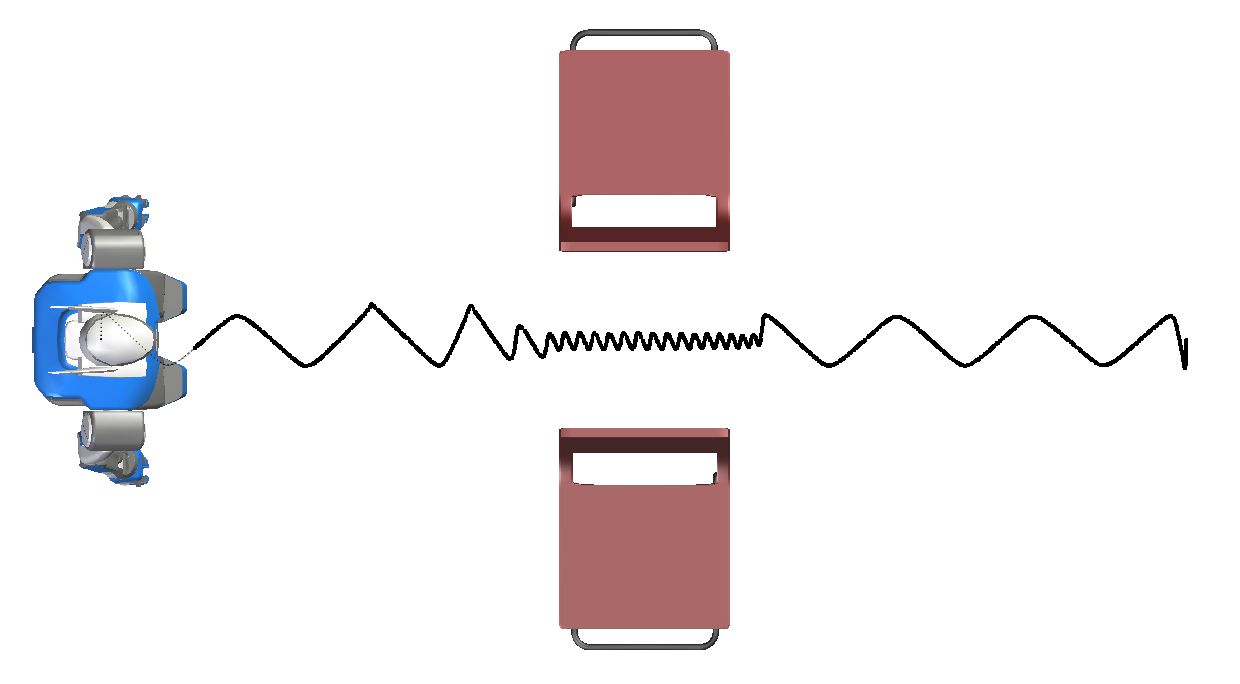
\includegraphics[width=0.7\linewidth]{pics/chairs/waist-trajectory.png}

\caption{Horizontal trajectory of the robot CoM during
  locomotion. When the robot is close to obstacles, the amplitude of
  the oscillations decreases.}
\label{fig:chairs-waist}
\end{figure}



Fig.  \ref{fig:chairs-waist} shows  the horizontal  trajectory  of the
robot CoM  during  locomotion. The amplitude of the oscillations  decreases when passing
between the  chairs.  This motion has  been validated on  a real HRP-2
platform. Extension 2 shows a video of the experiment.


\subsection{Walking among floating obstacles}

\begin{figure}[h!]

\centering

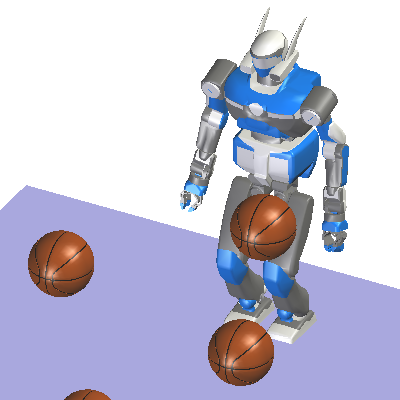
\includegraphics[width=0.24\linewidth]{pics/objects-cloud/perspective-1.png}
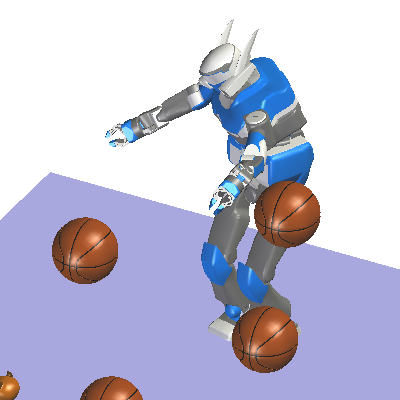
\includegraphics[width=0.24\linewidth]{pics/objects-cloud/perspective-2.png}
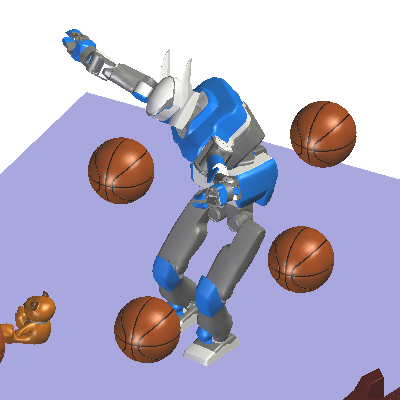
\includegraphics[width=0.24\linewidth]{pics/objects-cloud/perspective-3.png}
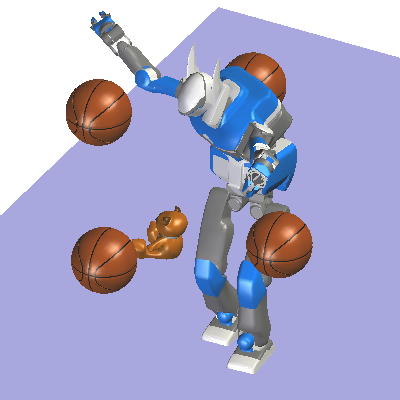
\includegraphics[width=0.24\linewidth]{pics/objects-cloud/perspective-4.png}
\\ 
\vskip 0.08cm
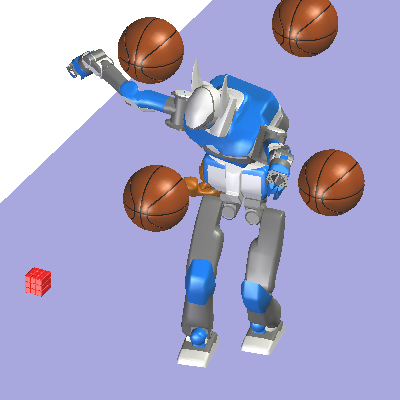
\includegraphics[width=0.24\linewidth]{pics/objects-cloud/perspective-5.png}
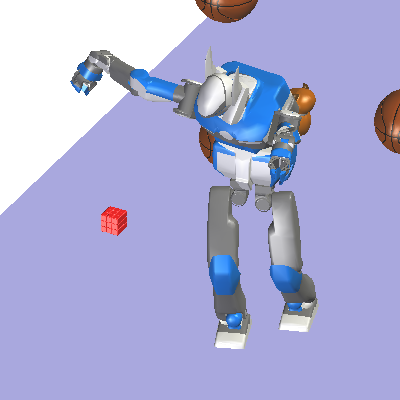
\includegraphics[width=0.24\linewidth]{pics/objects-cloud/perspective-6.png}
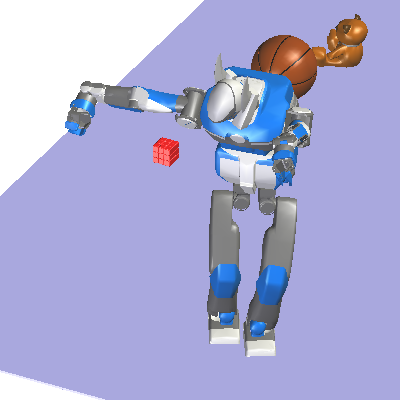
\includegraphics[width=0.24\linewidth]{pics/objects-cloud/perspective-7.png}
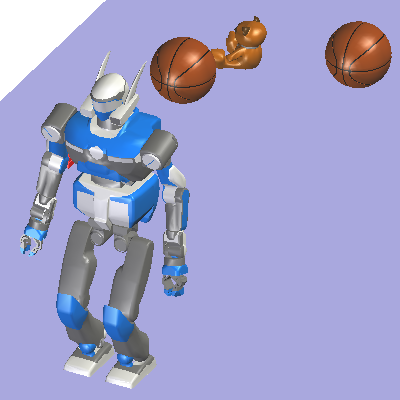
\includegraphics[width=0.24\linewidth]{pics/objects-cloud/perspective-8.png}

\caption{Solution path for a cluttered environment, the robot walks
  among floating obstacles.}
\label{fig:cluttered}
\end{figure}

In the environment shown in Fig. \ref{fig:cluttered}, the robot
has to find a way among floating obstacles. In this
environment neither bounding box nor footstep planning strategies
could find a collision-free walk trajectory.
The first planning stage requires
53~s on average, and the animation of the trajectory presented in 
Fig.~\ref{fig:cluttered} uses 339.5~s of computation time. Fig.~\ref{fig:cluttered-waist} 
shows the robot CoM trajectory during locomotion.

\begin{figure}[h!]
  \centering
  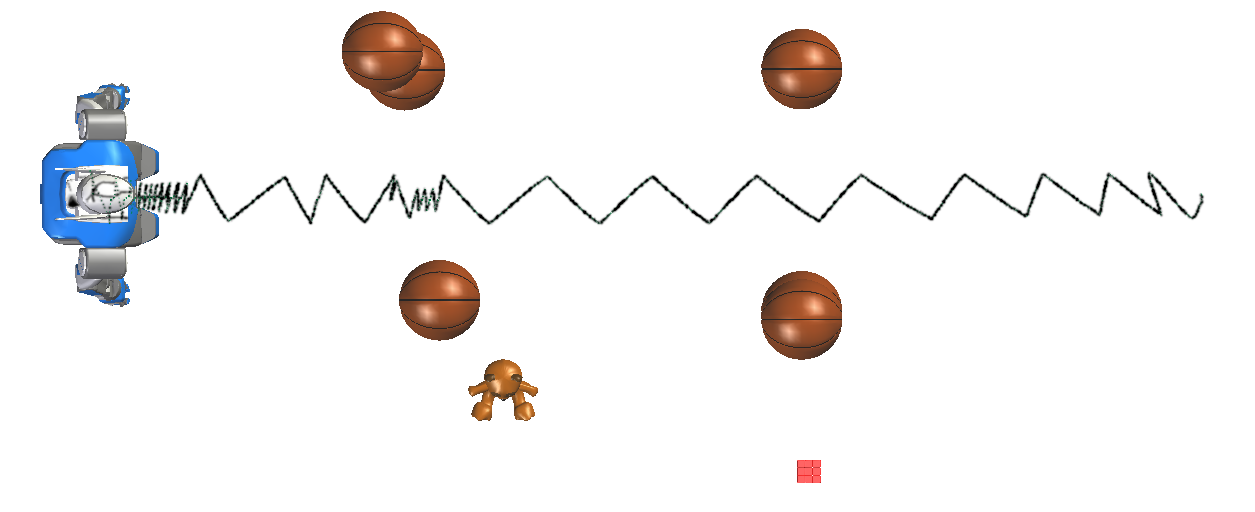
\includegraphics[width=0.7\linewidth]{pics/objects-cloud/waist-trajectory.png}

  \caption{Horizontal trajectory of the robot CoM during
    locomotion.}
  \label{fig:cluttered-waist} 
\end{figure}


\subsection{'Put the ball on a shelf'}
\label{sec:shelf}

In the problem shown in Fig. \ref{fig:shelf} the robot has to put a ball on a
shelf, in a constrained apartment environment. The final configuration is defined 
implicitly as a desired hand position. We have generated automatically goal configurations 
solving the task, as described in Section~\ref{sec:wb} . Then, we have
applied our planner to generate a whole-body walking motion that solves the hand reaching
task. 

The solution sliding path is constrained between the table on the right and the lamp
on the left. This passage is too narrow for the robot nominal walk parameters. 
When executing the walk motion resulting from our algorithm, the robot left hand
is only a few centimeters away from the lamp.

\textbf{The first planning stage requires 15~s on average, and the
  animation of the resulting walk motion presented in
  Fig.~\ref{fig:shelf} requires around 190~s of computation time.}
Fig.~\ref{fig:shelf-waist} shows the robot CoM trajectory during
locomotion. Extension 3 presents a comprehensive video of this
problem, including the motion execution on the real robot HRP-2 on
stage. Fig.~\ref{fig:shelf-cdf} shows some snapshots taken from
Extension 3.


\begin{figure}[h]
\centering
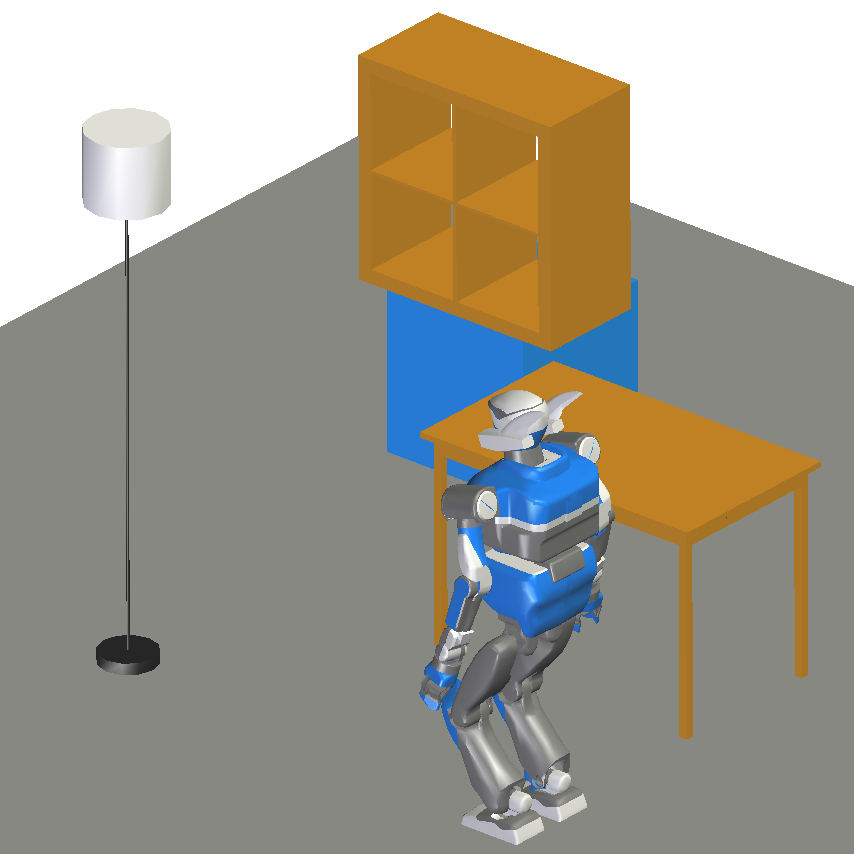
\includegraphics[width=0.24\linewidth]{pics/shelves/trajectory-1.png}
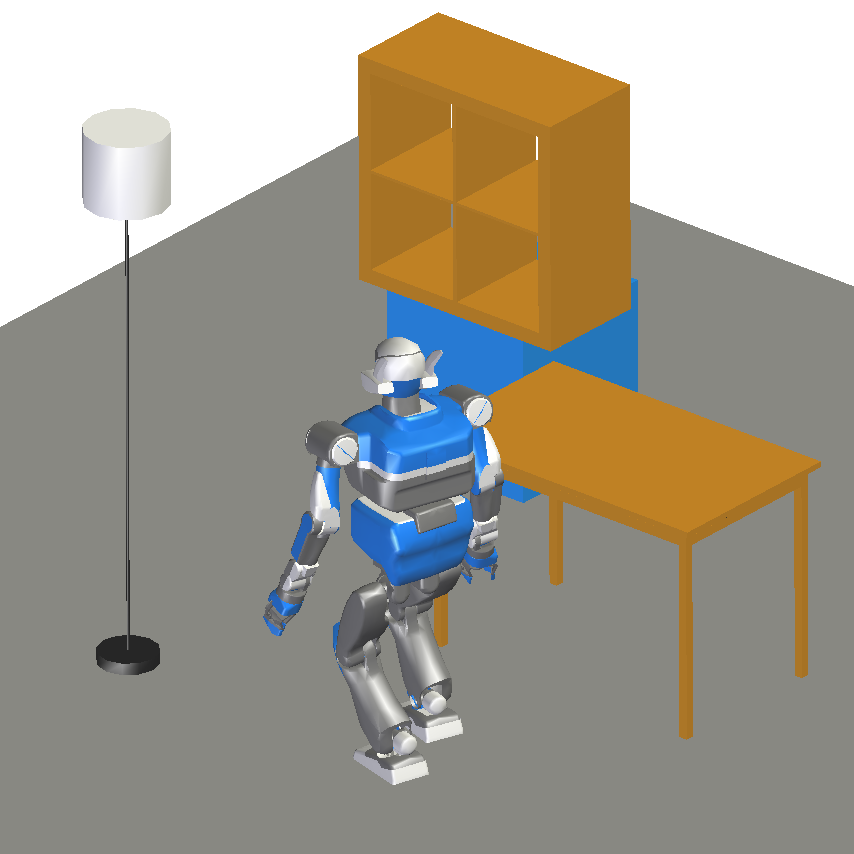
\includegraphics[width=0.24\linewidth]{pics/shelves/trajectory-2.png}
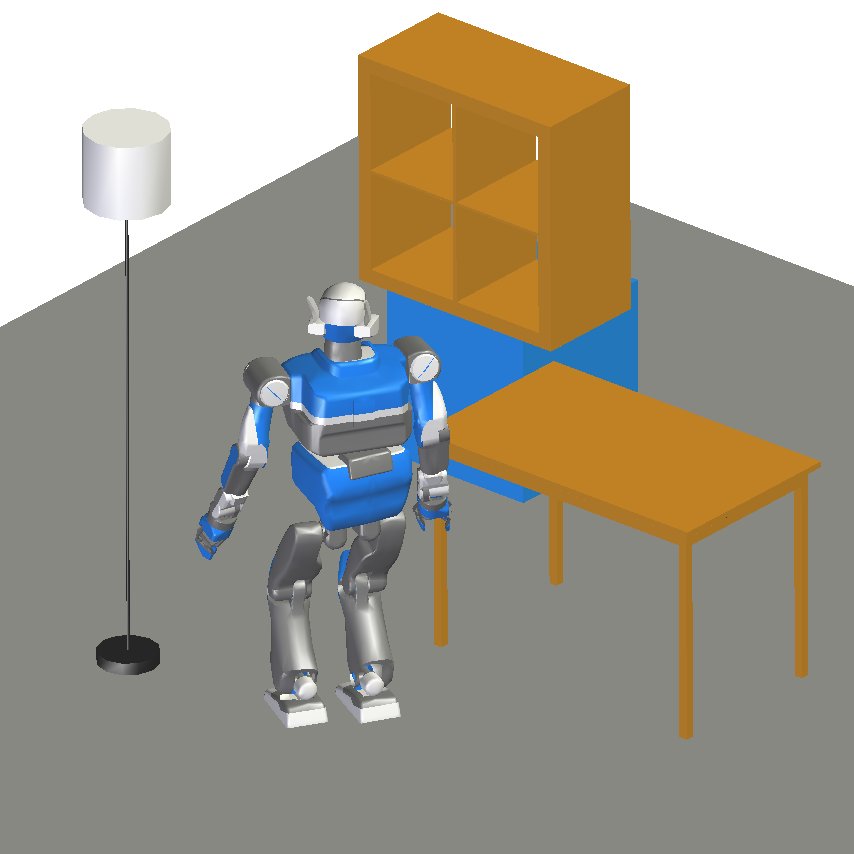
\includegraphics[width=0.24\linewidth]{pics/shelves/trajectory-3.png}
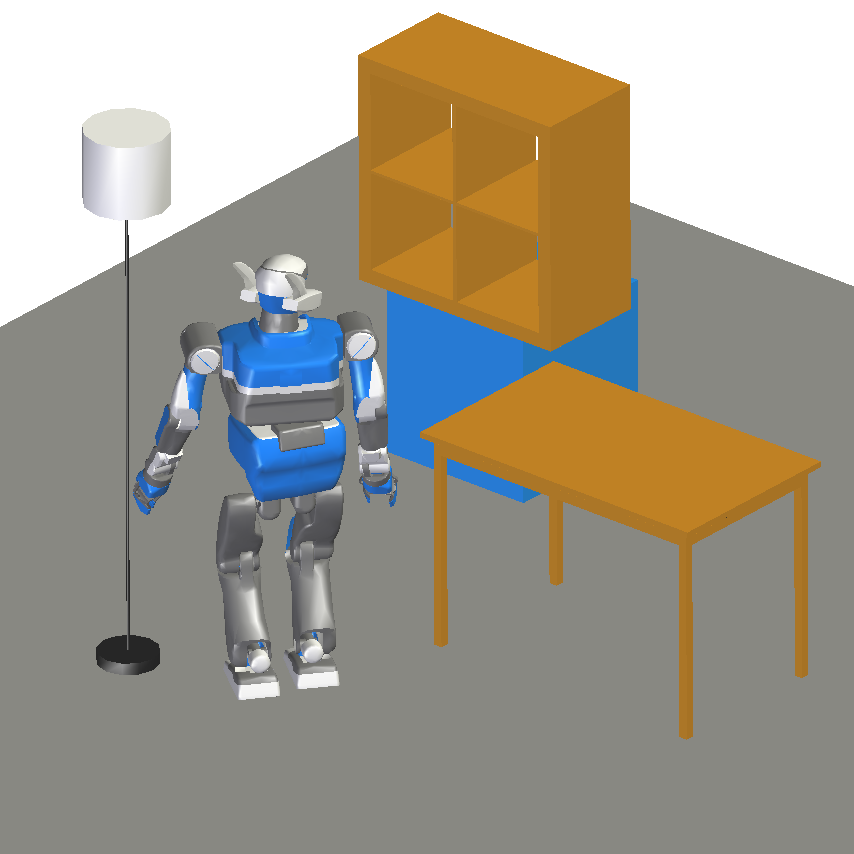
\includegraphics[width=0.24\linewidth]{pics/shelves/trajectory-4.png}
\\ 
\vskip 0.1cm
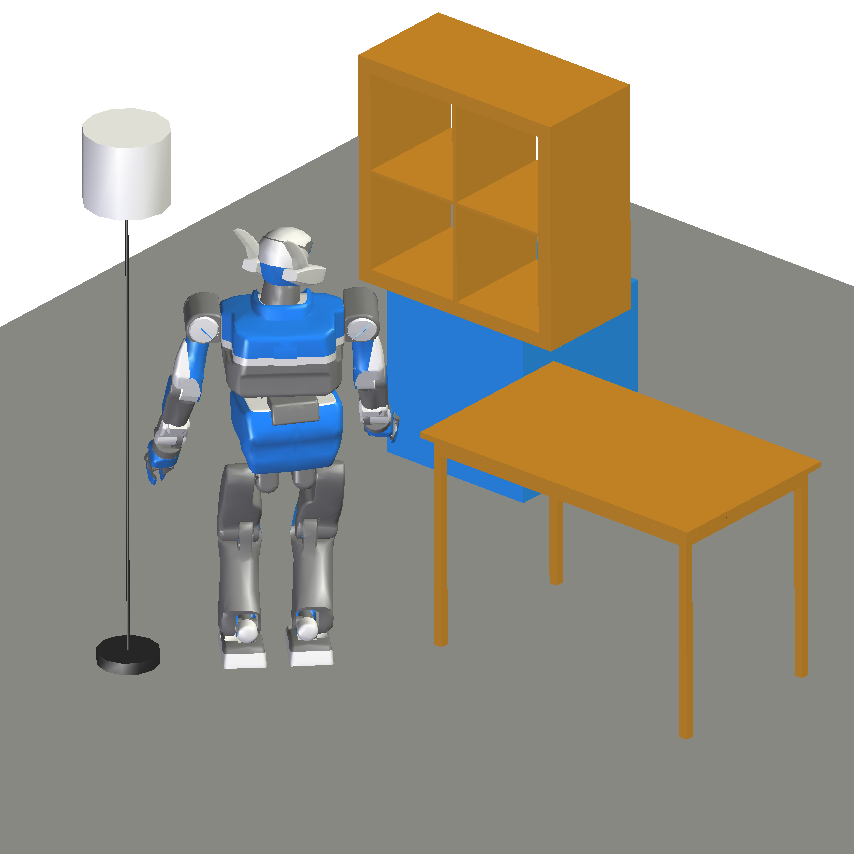
\includegraphics[width=0.24\linewidth]{pics/shelves/trajectory-5.png}
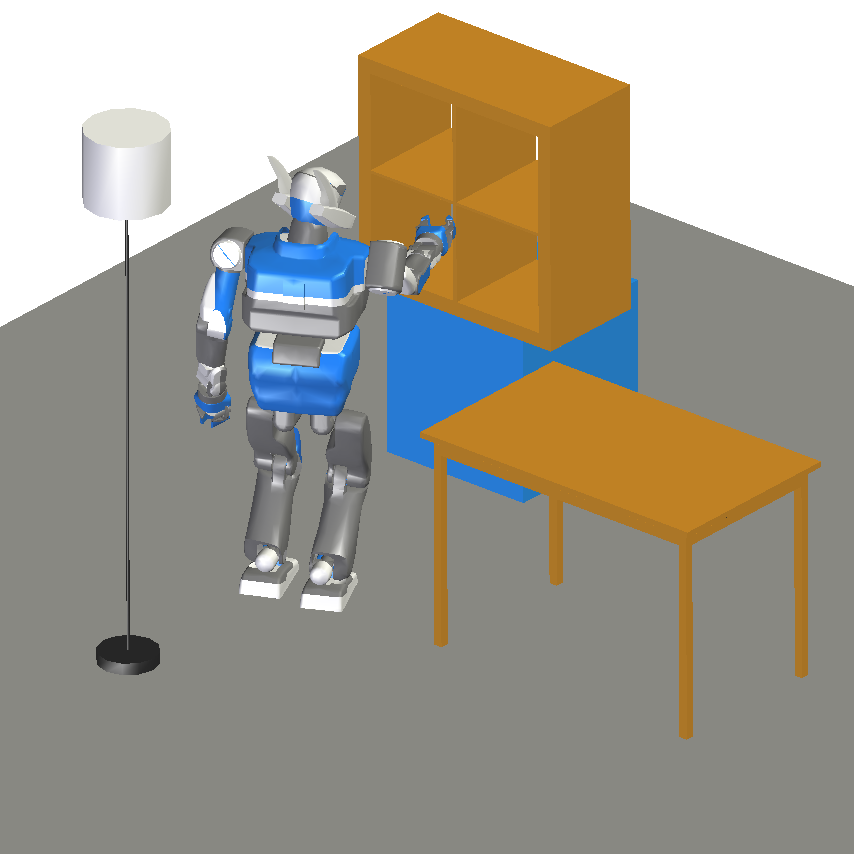
\includegraphics[width=0.24\linewidth]{pics/shelves/trajectory-6.png}
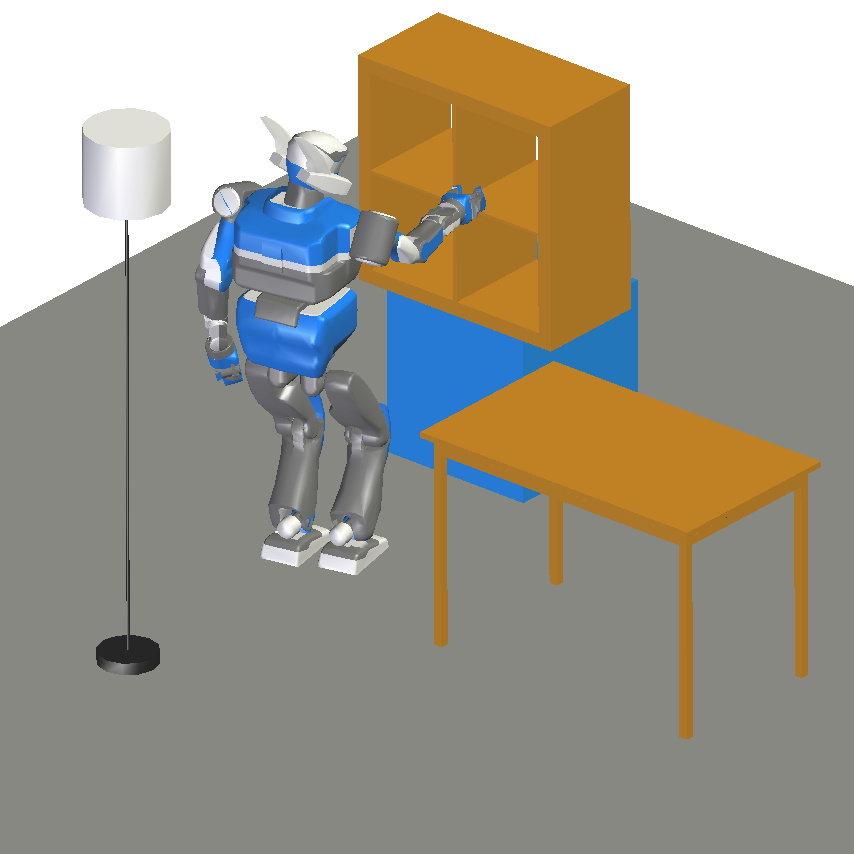
\includegraphics[width=0.24\linewidth]{pics/shelves/trajectory-7.png}
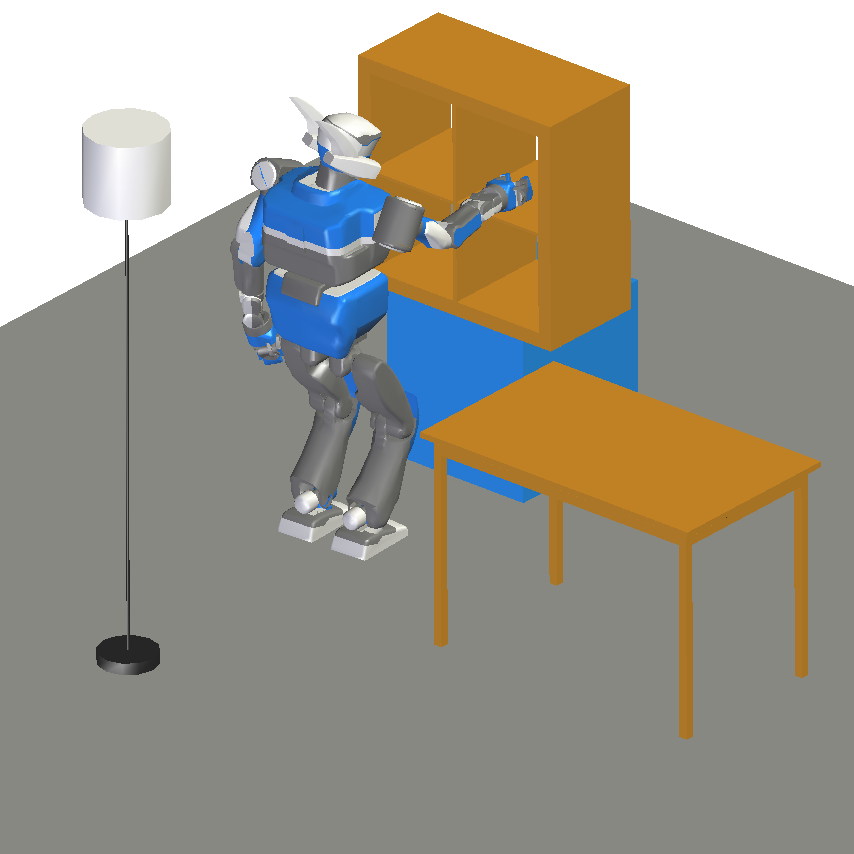
\includegraphics[width=0.24\linewidth]{pics/shelves/trajectory-8.png}

\caption{Solution path for a hand reaching problem in an
  apartment. The goal is implicitly defined as an inverse kinematics
  task.} 
\label{fig:shelf}
\end{figure}




\begin{figure}[h]
\centering

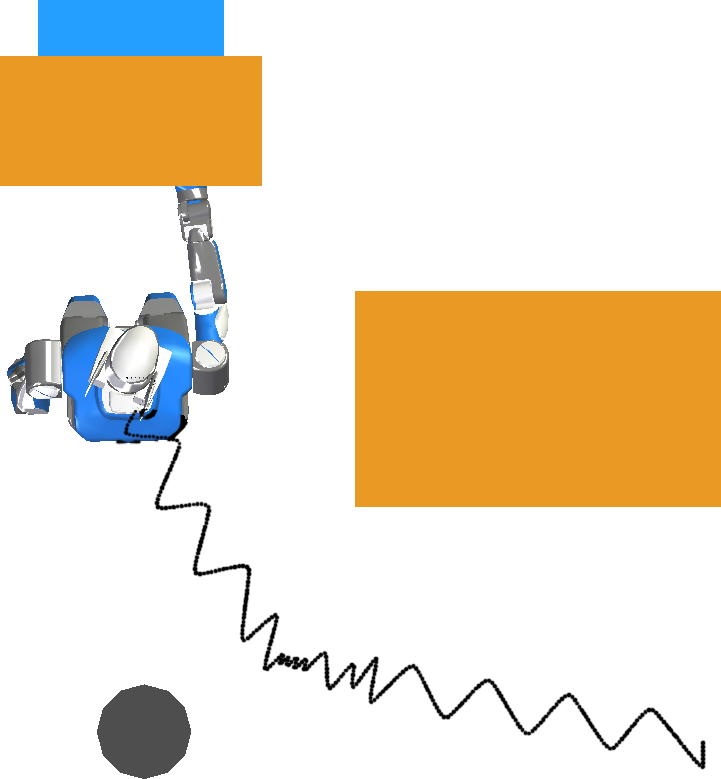
\includegraphics[width=0.4\linewidth]{pics/shelves/waist-trajectory.png}


\caption{Horizontal trajectory of the robot CoM during
    locomotion.}
\label{fig:shelf-waist}
\end{figure}

\begin{figure}[h]
\centering

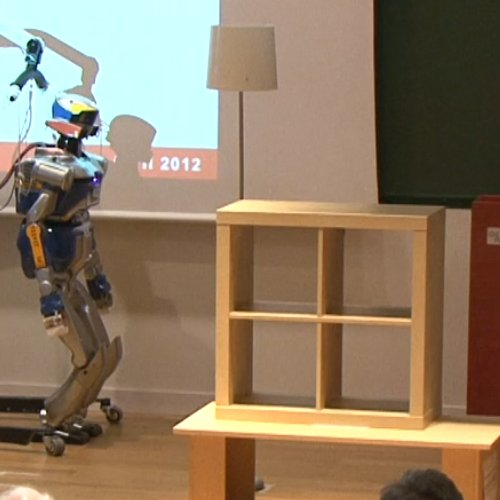
\includegraphics[width=0.19\linewidth]{pics/shelves-cdf/1.jpg}
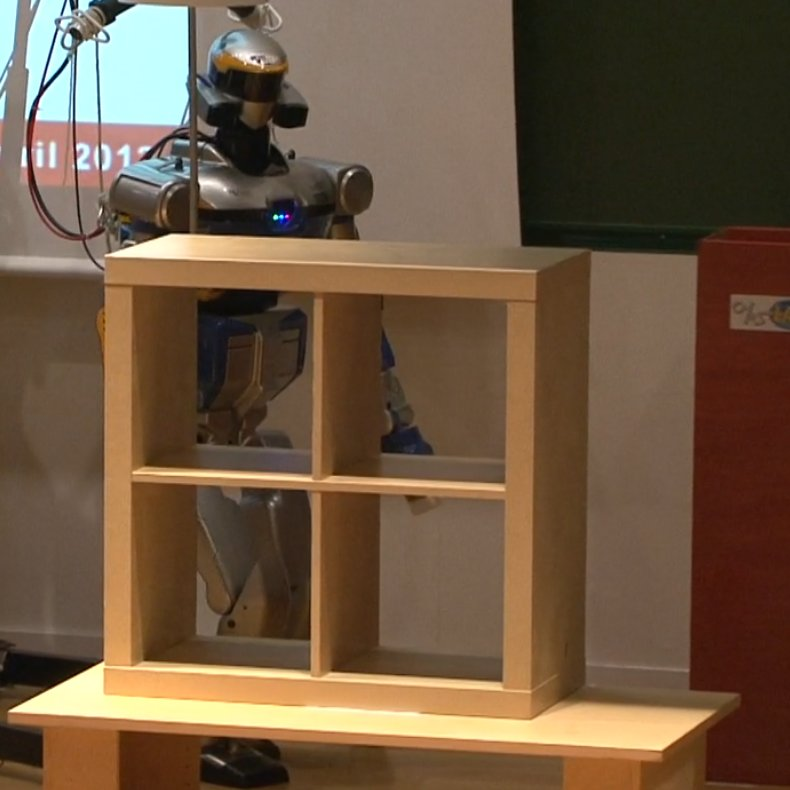
\includegraphics[width=0.19\linewidth]{pics/shelves-cdf/2.jpg}
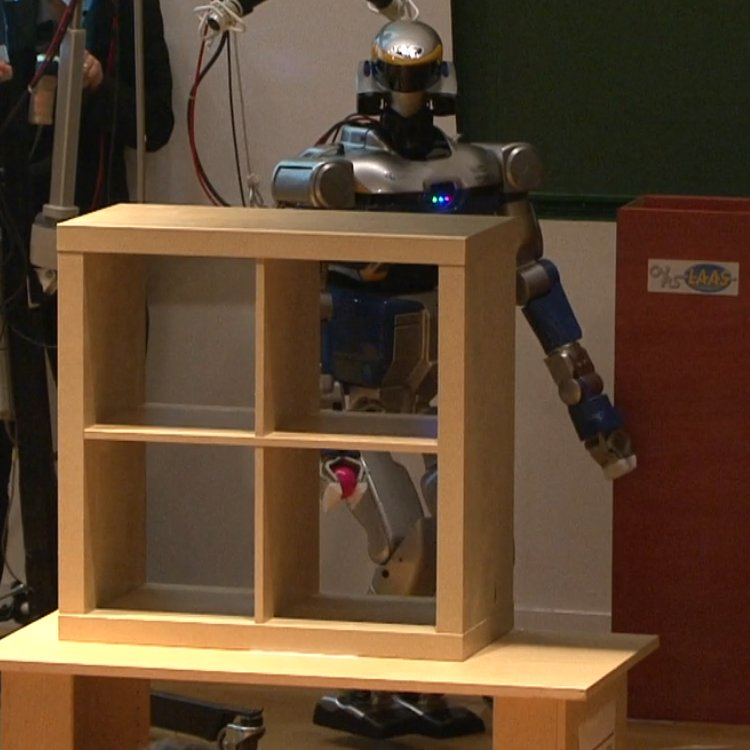
\includegraphics[width=0.19\linewidth]{pics/shelves-cdf/3.jpg}
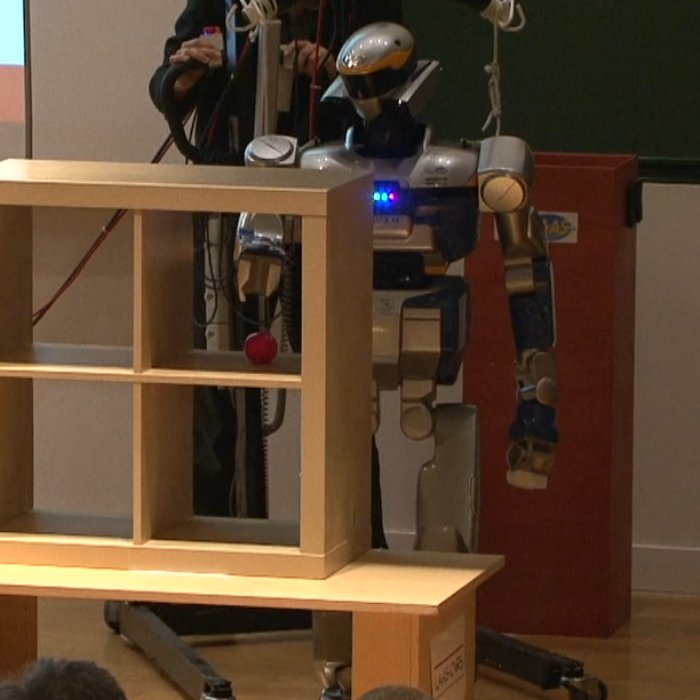
\includegraphics[width=0.19\linewidth]{pics/shelves-cdf/4.jpg}
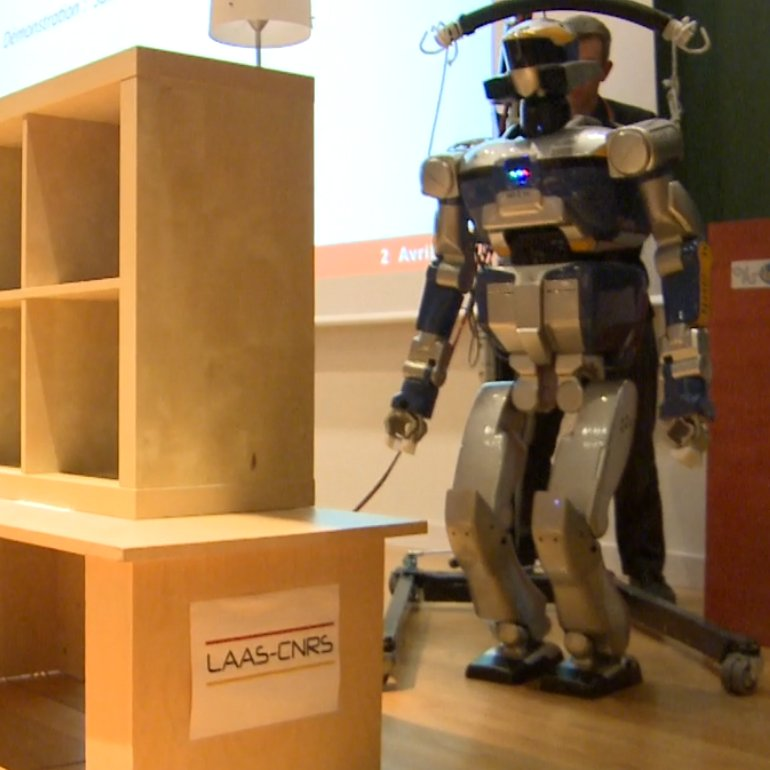
\includegraphics[width=0.19\linewidth]{pics/shelves-cdf/5.jpg}

\caption{Execution of the walking trajectory by HRP-2 on stage. The robot first goes
  to the shelves to release the ball, then comes back to a rest position.}

\label{fig:shelf-cdf}
\end{figure}

\section{Limits and Discussions}
\label{sec:limits}

This section lists several limitations of the current methods, and discusses
potential future work to overcome them.


\subsection{Stepping over obstacles}

Because of the kinematic constraints we apply at the planning stage, we are not
able yet to plan motions where the robot steps over obstacles, while this is an 
important feature of humanoid robots. Nevertheless, because we compute collision queries on
an exact model of the robot, our method is able to generate paths where obstacles
pass between the feet of the robot.
In future work, we plan to develop mixed
methods, where collision avoidance at the leg level can be solved by footstep
planning techniques, while whole-body collision-avoidance can be solved by the
algorithm presented in this paper.

\subsection{Environment representation}

\textbf{The experimental setup assumes perfect knowledge of the
  environment. This can be guaranteed during experiments by using
  calibrated objects and motion capture systems. This indeed allows us
  to focus on complex motion planning problems. The perception
  problem, interesting as it is, is thus completely decoupled from the
  planning problem in our presentation. From previous experiences
  however, we are confident that our algorithm will work as well in
  environments modeled by vision \cite{Nakhei4755945,DanLauLam2012}.}

\subsection{Trajectory following}

The setup also assumes perfect execution of the plan. It can be
critical here, since non-nominal stepping may cause the robot to drift
away from the planned trajectory. Future experiments will include
trajectory following during plan execution.

\section{Conclusion}

In this paper, we have presented a simple algorithm for constrained motion planning
and used it within a novel, well-grounded strategy for humanoid whole-body
manipulation planning including locomotion. The locomotion algorithm is based on a formal
small-space controllability property of humanoid robots. An important point is that
this strategy only holds for dynamic walking robots, and not for quasi-static walking ones.
We have used our motion planner on different challenging examples, and validated the
generated motions on a real platform. We have discussed the limits and potential extensions
of our method, and we plan to address them in future work.

\section{Acknowledgments}

This work was supported by the French FUI Project ROMEO and the European Project ECHORD-231143. The authors would like to thank Thomas Moulard and Olivier Stasse for their valuable help during experiments.

\appendix
\section{Sliding Motion Planning Benchmarks}
\label{app:bench}

\begin{figure}[H]
\centering
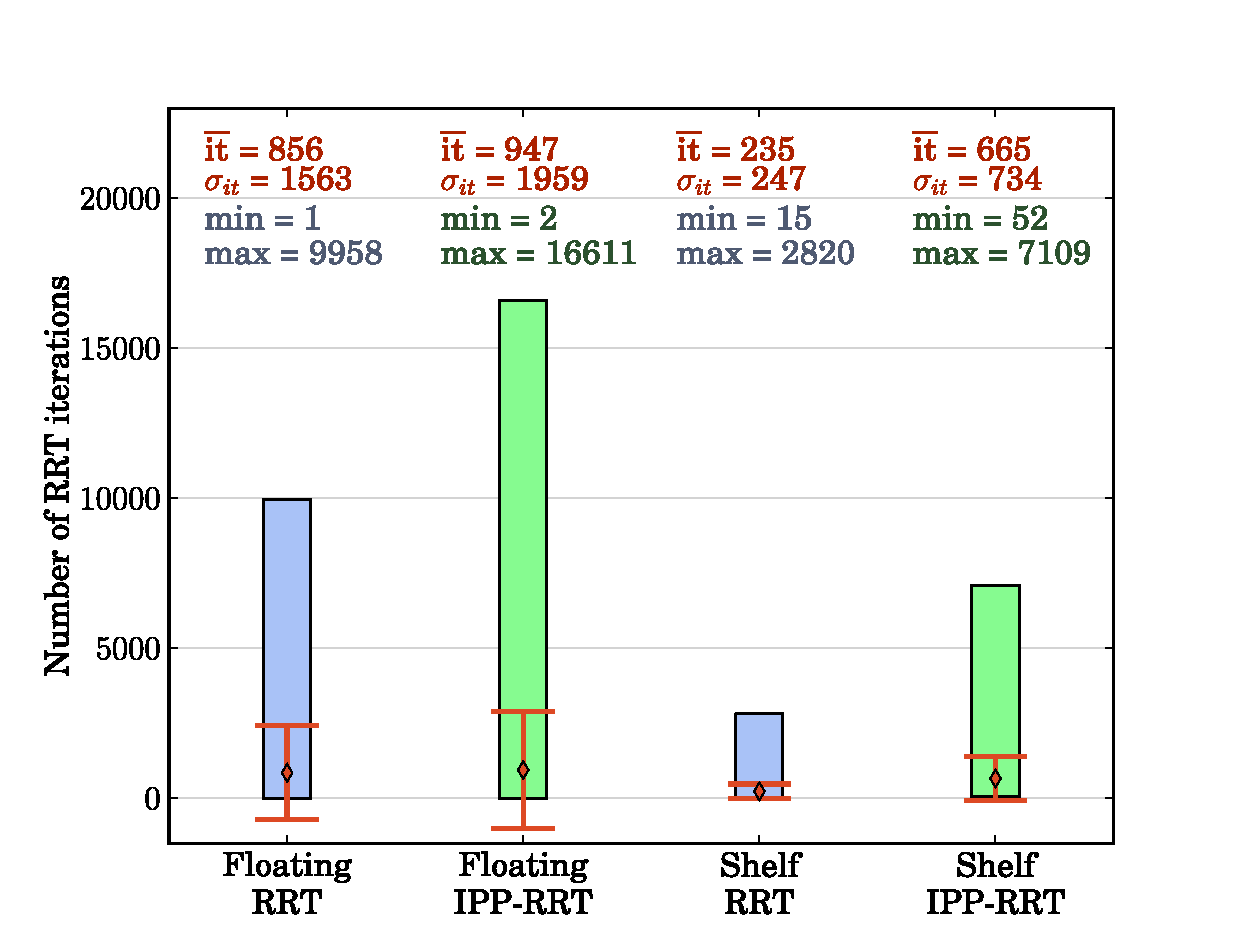
\includegraphics[width=0.8\linewidth]{plots/rrt-it.eps}
\caption{Number of RRT iterations $it$ for the floating objects and the
  shelf scenarios, using two variants of RRT. Mean $\overline{it}$,
  standard deviation $\sigma_{it}$, minimum and maximum values are
  represented.}
\label{fig:rrt-it}
\end{figure}

\begin{figure}[H]
\centering
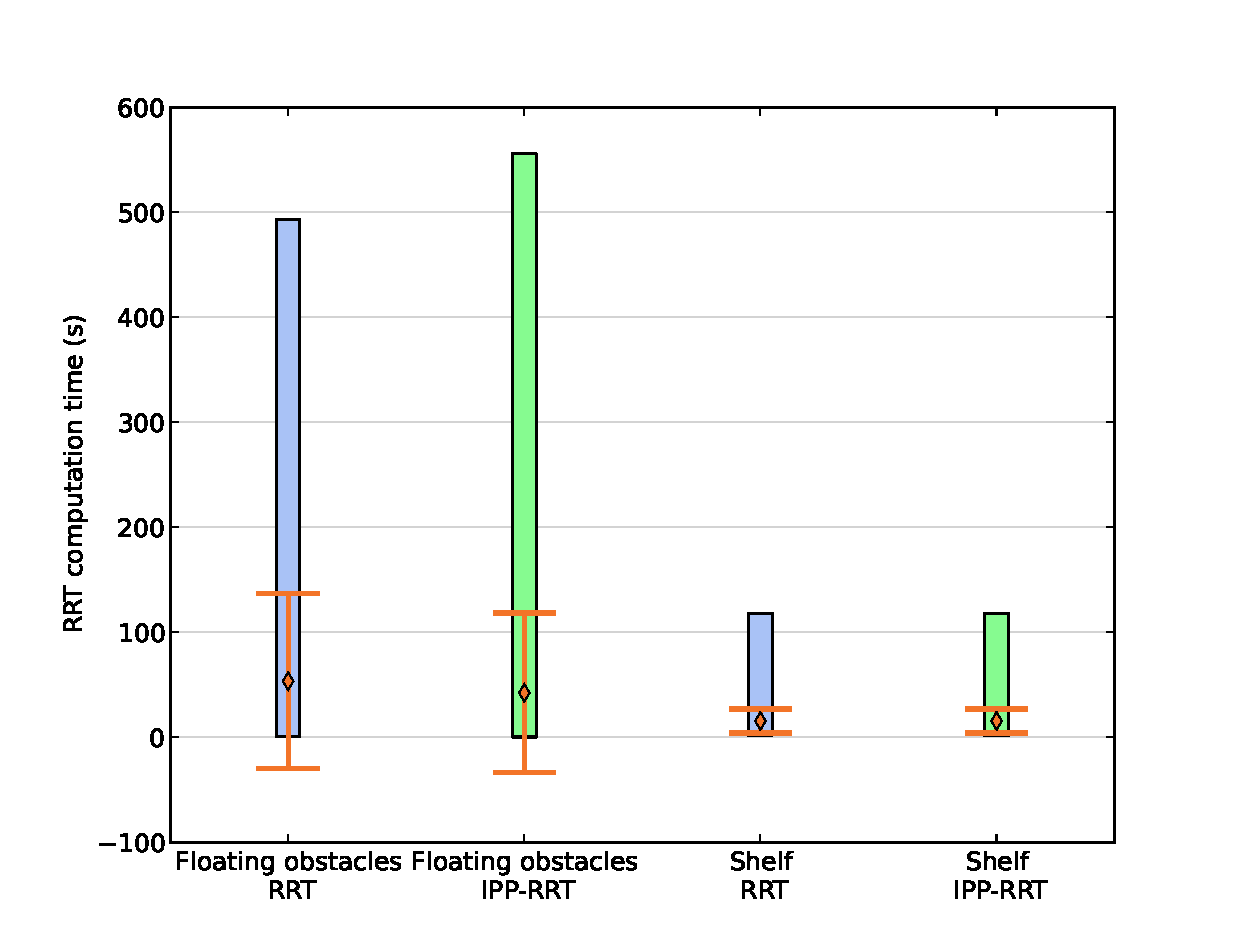
\includegraphics[width=0.8\linewidth]{plots/rrt-t.eps}
\caption{RRT computation time $t$ for the floating objects and the shelf
  scenarios, using two variants of RRT. Mean $\overline{t}$, standard
  deviation $\sigma_{t}$, minimum and maximum values are represented.}
\label{fig:rrt-t}
\end{figure}

\begin{figure}[H]
\centering
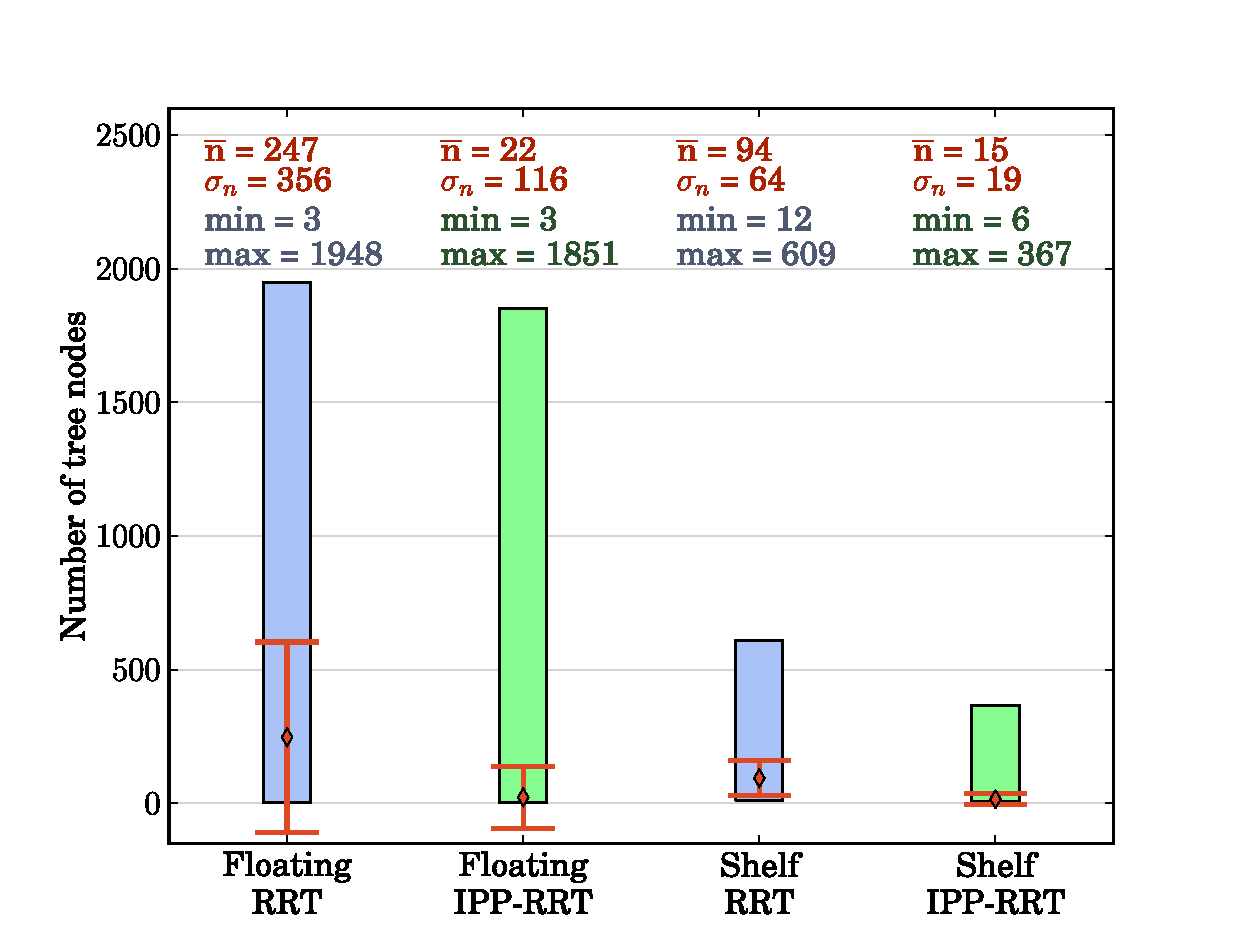
\includegraphics[width=0.8\linewidth]{plots/rrt-n.eps}
\caption{Number of tree nodes $n$ for the floating objects and the
  shelf scenarios, using two variants of RRT. Mean $\overline{n}$,
  standard deviation $\sigma_{n}$, minimum and maximum values are
  represented.}
\label{fig:rrt-n}
\end{figure}

\section{Index to Multimedia Extensions}

\begin{table}[H]
\begin{tabular}{c c m{0.7\linewidth}}
\hline
Extension & Type & Description \\
\hline
1 & Video & Example of a constrained motion planning result executed
on HRP-2. \\
2 & Video & Chairs scenario: solution of whole-body planning executed
on HRP-2. \\
3 & Video & Shelf scenario: solution of whole-body planning executed
in simulation and on HRP-2. \\
4 & Data & Raw data of sliding motion planning benchmarks for all
scenarios. \\
\hline
\end{tabular}
\end{table}

\bibliographystyle{agsm}   


\bibliography{bibli}



\end{document}
